%%
%% Copyright 2007, 2008, 2009 Elsevier Ltd
%%
%% This file is part of the 'Elsarticle Bundle'.
%% ---------------------------------------------
%%
%% It may be distributed under the conditions of the LaTeX Project Public
%% License, either version 1.2 of this license or (at your option) any
%% later version.  The latest version of this license is in
%%    http://www.latex-project.org/lppl.txt
%% and version 1.2 or later is part of all distributions of LaTeX
%% version 1999/12/01 or later.
%%
%% The list of all files belonging to the 'Elsarticle Bundle' is
%% given in the file `manifest.txt'.
%%

%% Template article for Elsevier's document class `elsarticle'
%% with harvard style bibliographic references
%% SP 2008/03/01
%%
%%
%%
%% $Id: elsarticle-template-harv.tex 4 2009-10-24 08:22:58Z rishi $
%%
%%
\documentclass[preprint,authoryear,12pt]{elsarticle}

%% Use the option review to obtain double line spacing
%% \documentclass[authoryear,preprint,review,12pt]{elsarticle}

%% Use the options 1p,twocolumn; 3p; 3p,twocolumn; 5p; or 5p,twocolumn
%% for a journal layout:
%% \documentclass[final,authoryear,1p,times]{elsarticle}
%% \documentclass[final,authoryear,1p,times,twocolumn]{elsarticle}
%% \documentclass[final,authoryear,3p,times]{elsarticle}
%% \documentclass[final,authoryear,3p,times,twocolumn]{elsarticle}
%% \documentclass[final,authoryear,5p,times]{elsarticle}
%% \documentclass[final,authoryear,5p,times,twocolumn]{elsarticle}

%% if you use PostScript figures in your article
%% use the graphics package for simple commands
%% \usepackage{graphics}
%% or use the graphicx package for more complicated commands
\usepackage{graphicx}
%% or use the epsfig package if you prefer to use the old commands
%% \usepackage{epsfig}

%% The amssymb package provides various useful mathematical symbols
\usepackage{amssymb}
%% The amsthm package provides extended theorem environments
%% \usepackage{amsthm}

%% The lineno packages adds line numbers. Start line numbering with
%% \begin{linenumbers}, end it with \end{linenumbers}. Or switch it on
%% for the whole article with \linenumbers after \end{frontmatter}.
%% \usepackage{lineno}

%% natbib.sty is loaded by default. However, natbib options can be
%% provided with \biboptions{...} command. Following options are
%% valid:

%%   round  -  round parentheses are used (default)
%%   square -  square brackets are used   [option]
%%   curly  -  curly braces are used      {option}
%%   angle  -  angle brackets are used    <option>
%%   semicolon  -  multiple citations separated by semi-colon (default)
%%   colon  - same as semicolon, an earlier confusion
%%   comma  -  separated by comma
%%   authoryear - selects author-year citations (default)
%%   numbers-  selects numerical citations
%%   super  -  numerical citations as superscripts
%%   sort   -  sorts multiple citations according to order in ref. list
%%   sort&compress   -  like sort, but also compresses numerical citations
%%   compress - compresses without sorting
%%   longnamesfirst  -  makes first citation full author list
%%
%% \biboptions{longnamesfirst,comma}

% \biboptions{}

\journal{Gene}

\begin{document}

\begin{frontmatter}

%% Title, authors and addresses

%% use the tnoteref command within \title for footnotes;
%% use the tnotetext command for the associated footnote;
%% use the fnref command within \author or \address for footnotes;
%% use the fntext command for the associated footnote;
%% use the corref command within \author for corresponding author footnotes;
%% use the cortext command for the associated footnote;
%% use the ead command for the email address,
%% and the form \ead[url] for the home page:
%%
%% \title{Title\tnoteref{label1}}
%% \tnotetext[label1]{}
%% \author{Name\corref{cor1}\fnref{label2}}
%% \ead{email address}
%% \ead[url]{home page}
%% \fntext[label2]{}
%% \cortext[cor1]{}
%% \address{Address\fnref{label3}}
%% \fntext[label3]{}

\title{Constuction of executable in silico models of network dynamics based on experimental data}

%% use optional labels to link authors explicitly to addresses:
%% \author[label1,label2]{<author name>}
%% \address[label1]{<address>}
%% \address[label2]{<address>}
\author[bioeng]{Jetse~Schoma}
\ead{j.scholma@utwente.nl}
\author[bioeng]{Ricardo~A.~Urquidi~Camacho}
\ead{rauc6788@hotmail.com}
\author[fmt]{Stefano~Schivo}
\ead{s.schivo@utwente.nl}
\author[bioeng]{Janine~N.~Post\corref{corresp}}
\ead{j.n.post@utwente.nl}
\address[bioeng]{Developmental BioEngineering, MIRA Institute for Biomedical Technology and Technical Medicine, University of Twente, 7522NH Enschede, The~Netherlands}
\address[fmt]{Formal Methods and Tools, Faculty of EEMCS, University of Twente, 7522NH Enschede, The~Netherlands}
\cortext[corresp]{Corresponding author at: Developmental BioEngineering, MIRA Institute for Biomedical Technology and Technical Medicine, University of Twente, P.O. Box 217, 7522NH Enschede, The~Netherlands. Tel.: +31 (0)53 489 4205}

\begin{abstract}
\input{abstract.tex}
\end{abstract}

\begin{keyword}
%% keywords here, in the form: keyword \sep keyword

%% MSC codes here, in the form: \MSC code \sep code
%% or \MSC[2008] code \sep code (2000 is the default)

\end{keyword}

\end{frontmatter}

% \linenumbers

%% main text
\section{Introduction}\label{sec:intro}
\input{introduction.tex}

\section{Materials and Methods}\label{sec:methods}
\input{tab.tex}


%FIRST EXAMPLE STYLE

\tikzset{titregris/.style =
{draw=gray, thick, fill=white, shading = exersicetitle, %
text=black!70, rectangle, rounded corners, right,minimum height=.7cm}}
\pgfdeclarehorizontalshading{exersicebackground}{100bp}
{color(0bp)=(green!20); color(100bp)=(black!5)}
\pgfdeclarehorizontalshading{exersicetitle}{100bp}
{color(0bp)=(green!20);color(100bp)=(blue!5!white)}
\makeatletter
\mdfdefinestyle{ANIMOstyle}{%
nobreak=true,
outerlinewidth=1em,outerlinecolor=white,%
leftmargin=-1em,rightmargin=-1em,%
middlelinewidth=1.2pt,roundcorner=5pt,linecolor=gray,
apptotikzsetting={\tikzset{mdfbackground/.append style ={%
shading = exersicebackground}}},
innertopmargin=1.2\baselineskip,
skipabove={\dimexpr0.5\baselineskip+\topskip\relax},
skipbelow={-1em},
needspace=3\baselineskip,
frametitlefont=\sffamily\bfseries,
singleextra={%
\node[titregris,xshift=0.5cm] at (P-|O) %
{~\mdf@frametitlefont{\small What is ANIMO?}\hbox{~}};},
}
\makeatother

\begin{mdframed}[style=ANIMOstyle]
\pretolerance=2000
\scriptsize
ANIMO (Analysis of Networks with Interactive MOdeling)
is a software tool that allows the biologists to virtually \emph{play} with abstract network models.
Such models are based on cause-and-effect relationships, such as ``A activates B'', and their
behavior is described in semi-quantitative terms. This approach requires less precise knowledge about
kinetic parameters, while still enabling the user to easily investigate the dynamics of a modeled network.

The idea at the base of ANIMO is to provide experts with a means to visually represent their knowledge on biological interactions.
Networks created in this way are then enriched with simplified kinetics, producing \emph{dynamic models}.
Thanks to the Cytoscape-based user interface, the visual representation of a pathway available in ANIMO
closely resembles the networks commonly found in textbooks.

The network topology, equipped with informations
on its dynamic behavior, is automatically translated to an underlying formal model based on Timed Automata.
The formal model is used \emph{behind the scenes} to simulate the evolution of the network.
In a few seconds of computation, ANIMO presents the user with a graph plotting the levels of activation
of all components in the network during the simulation period.
A slider under the graph lets the user further explore the evolution of the model:
moving the slider makes the coloration of the network instantly reflect the activity of
all components along the simulation interval.
\end{mdframed}



%SECOND EXAMPLE


\mdfdefinestyle{ANIMObox}{%
    nobreak=true,
    outerlinecolor = gray!80!black,
    outerlinewidth=2pt,
    roundcorner=20pt,
    innertopmargin=\baselineskip,
    innerbottommargin=\baselineskip,
    innerrightmargin=10pt,
    innerleftmargin=10pt,
    backgroundcolor = gray!20!white}

\begin{mdframed}[style=ANIMObox]
{\bf Analysis of Networks with Interactive MOdeling}
\pretolerance=2000

\small
ANIMO is a software tool that allows the biologists to virtually \emph{play} with abstract network models.
Such models are based on cause-and-effect relationships, such as ``A activates B'', and their
behavior is described in semi-quantitative terms. This approach requires less precise knowledge about
kinetic parameters, while still enabling the user to easily investigate the dynamics of a modeled network.

The idea at the base of ANIMO is to provide experts with a means to visually represent their knowledge on biological interactions.
Networks created in this way are then enriched with simplified kinetics, producing \emph{dynamic models}.
Thanks to the Cytoscape-based user interface, the visual representation of a pathway available in ANIMO
closely resembles the networks commonly found in textbooks.

The network topology, equipped with informations
on its dynamic behavior, is automatically translated to an underlying formal model based on Timed Automata.
The formal model is used \emph{behind the scenes} to simulate the evolution of the network.
In a few seconds of computation, ANIMO presents the user with a graph plotting the levels of activation
of all components in the network during the simulation period.
A slider under the graph lets the user further explore the evolution of the model:
moving the slider makes the coloration of the network instantly reflect the activity of
all components along the simulation interval.
\end{mdframed}



\def\graphScale{0.0243}
\begin{figure*}[htbp]
\centering
\begin{tabular}{ll}
\subfloat[\label{fig:animo-settings-scenario-network}]{\includegraphics[scale=\graphScale]{scenario1-2_network_legend_CB}} &
\subfloat[\label{fig:animo-settings-scenario-graph}]{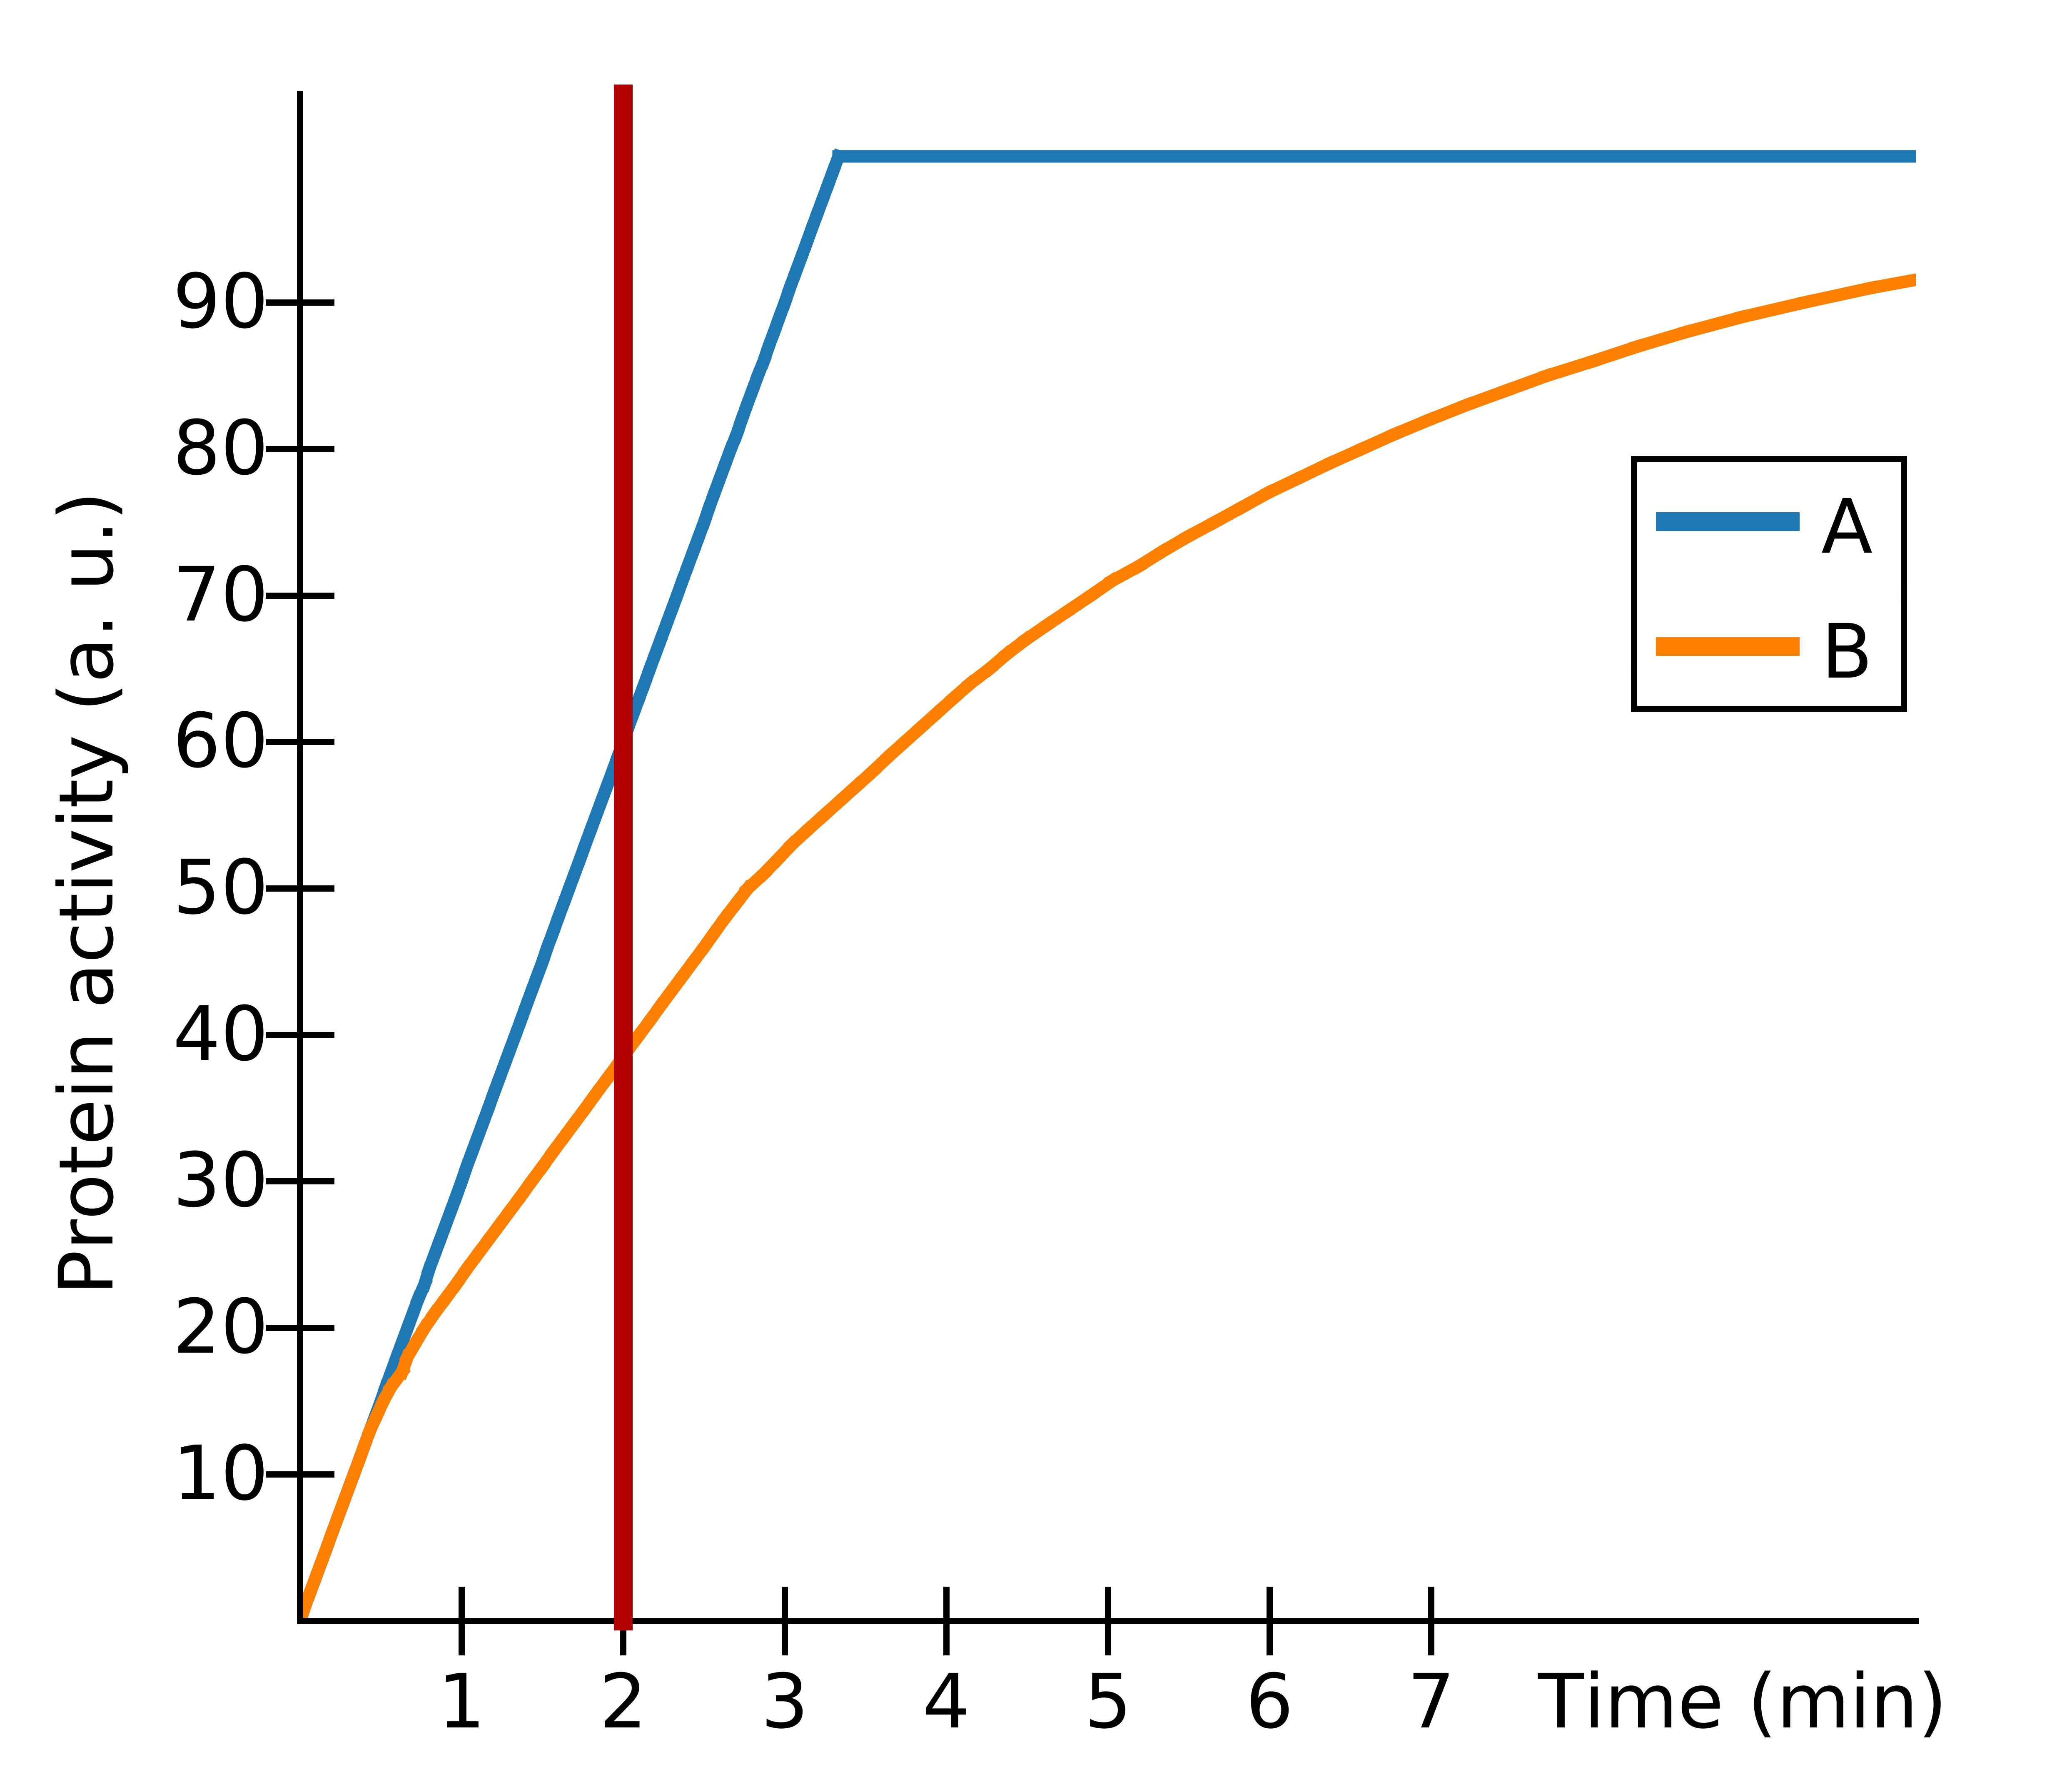
\includegraphics[scale=\graphScale]{scenario1-2_graph}} \\
\subfloat[\label{fig:animo-settings-k-network}]{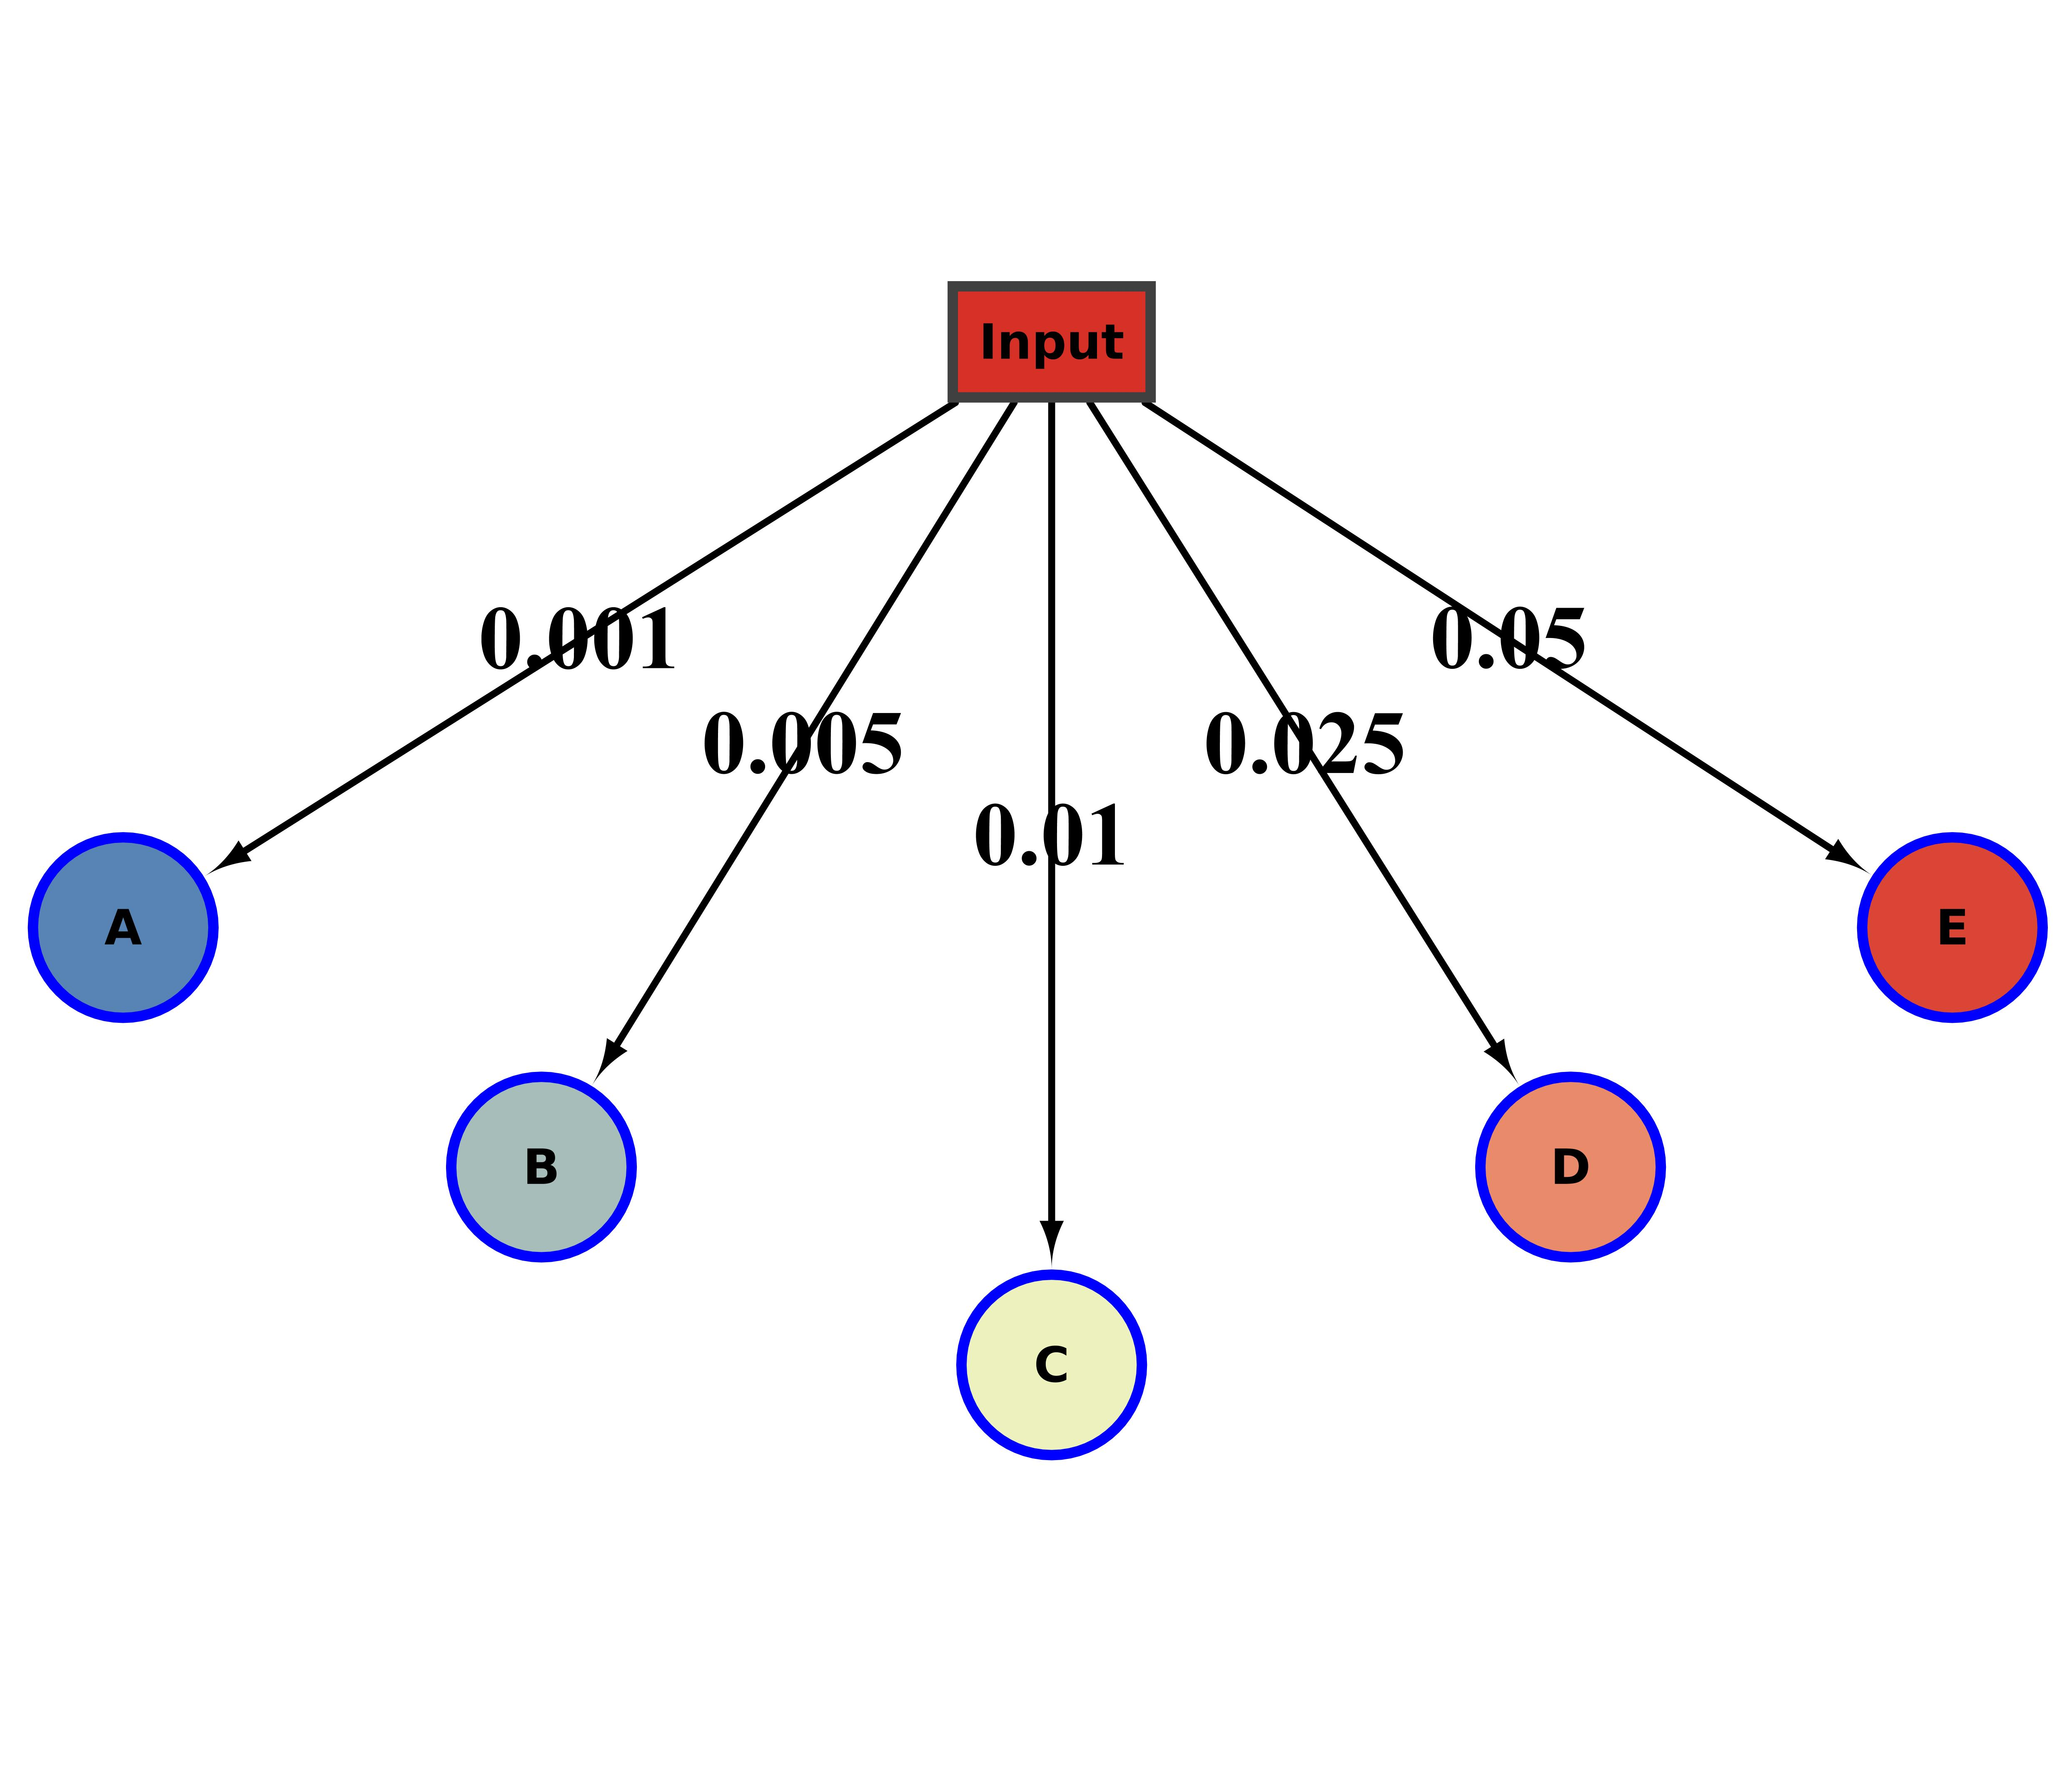
\includegraphics[scale=\graphScale]{parameter_network_CB}} &
\subfloat[\label{fig:animo-settings-k-graph}]{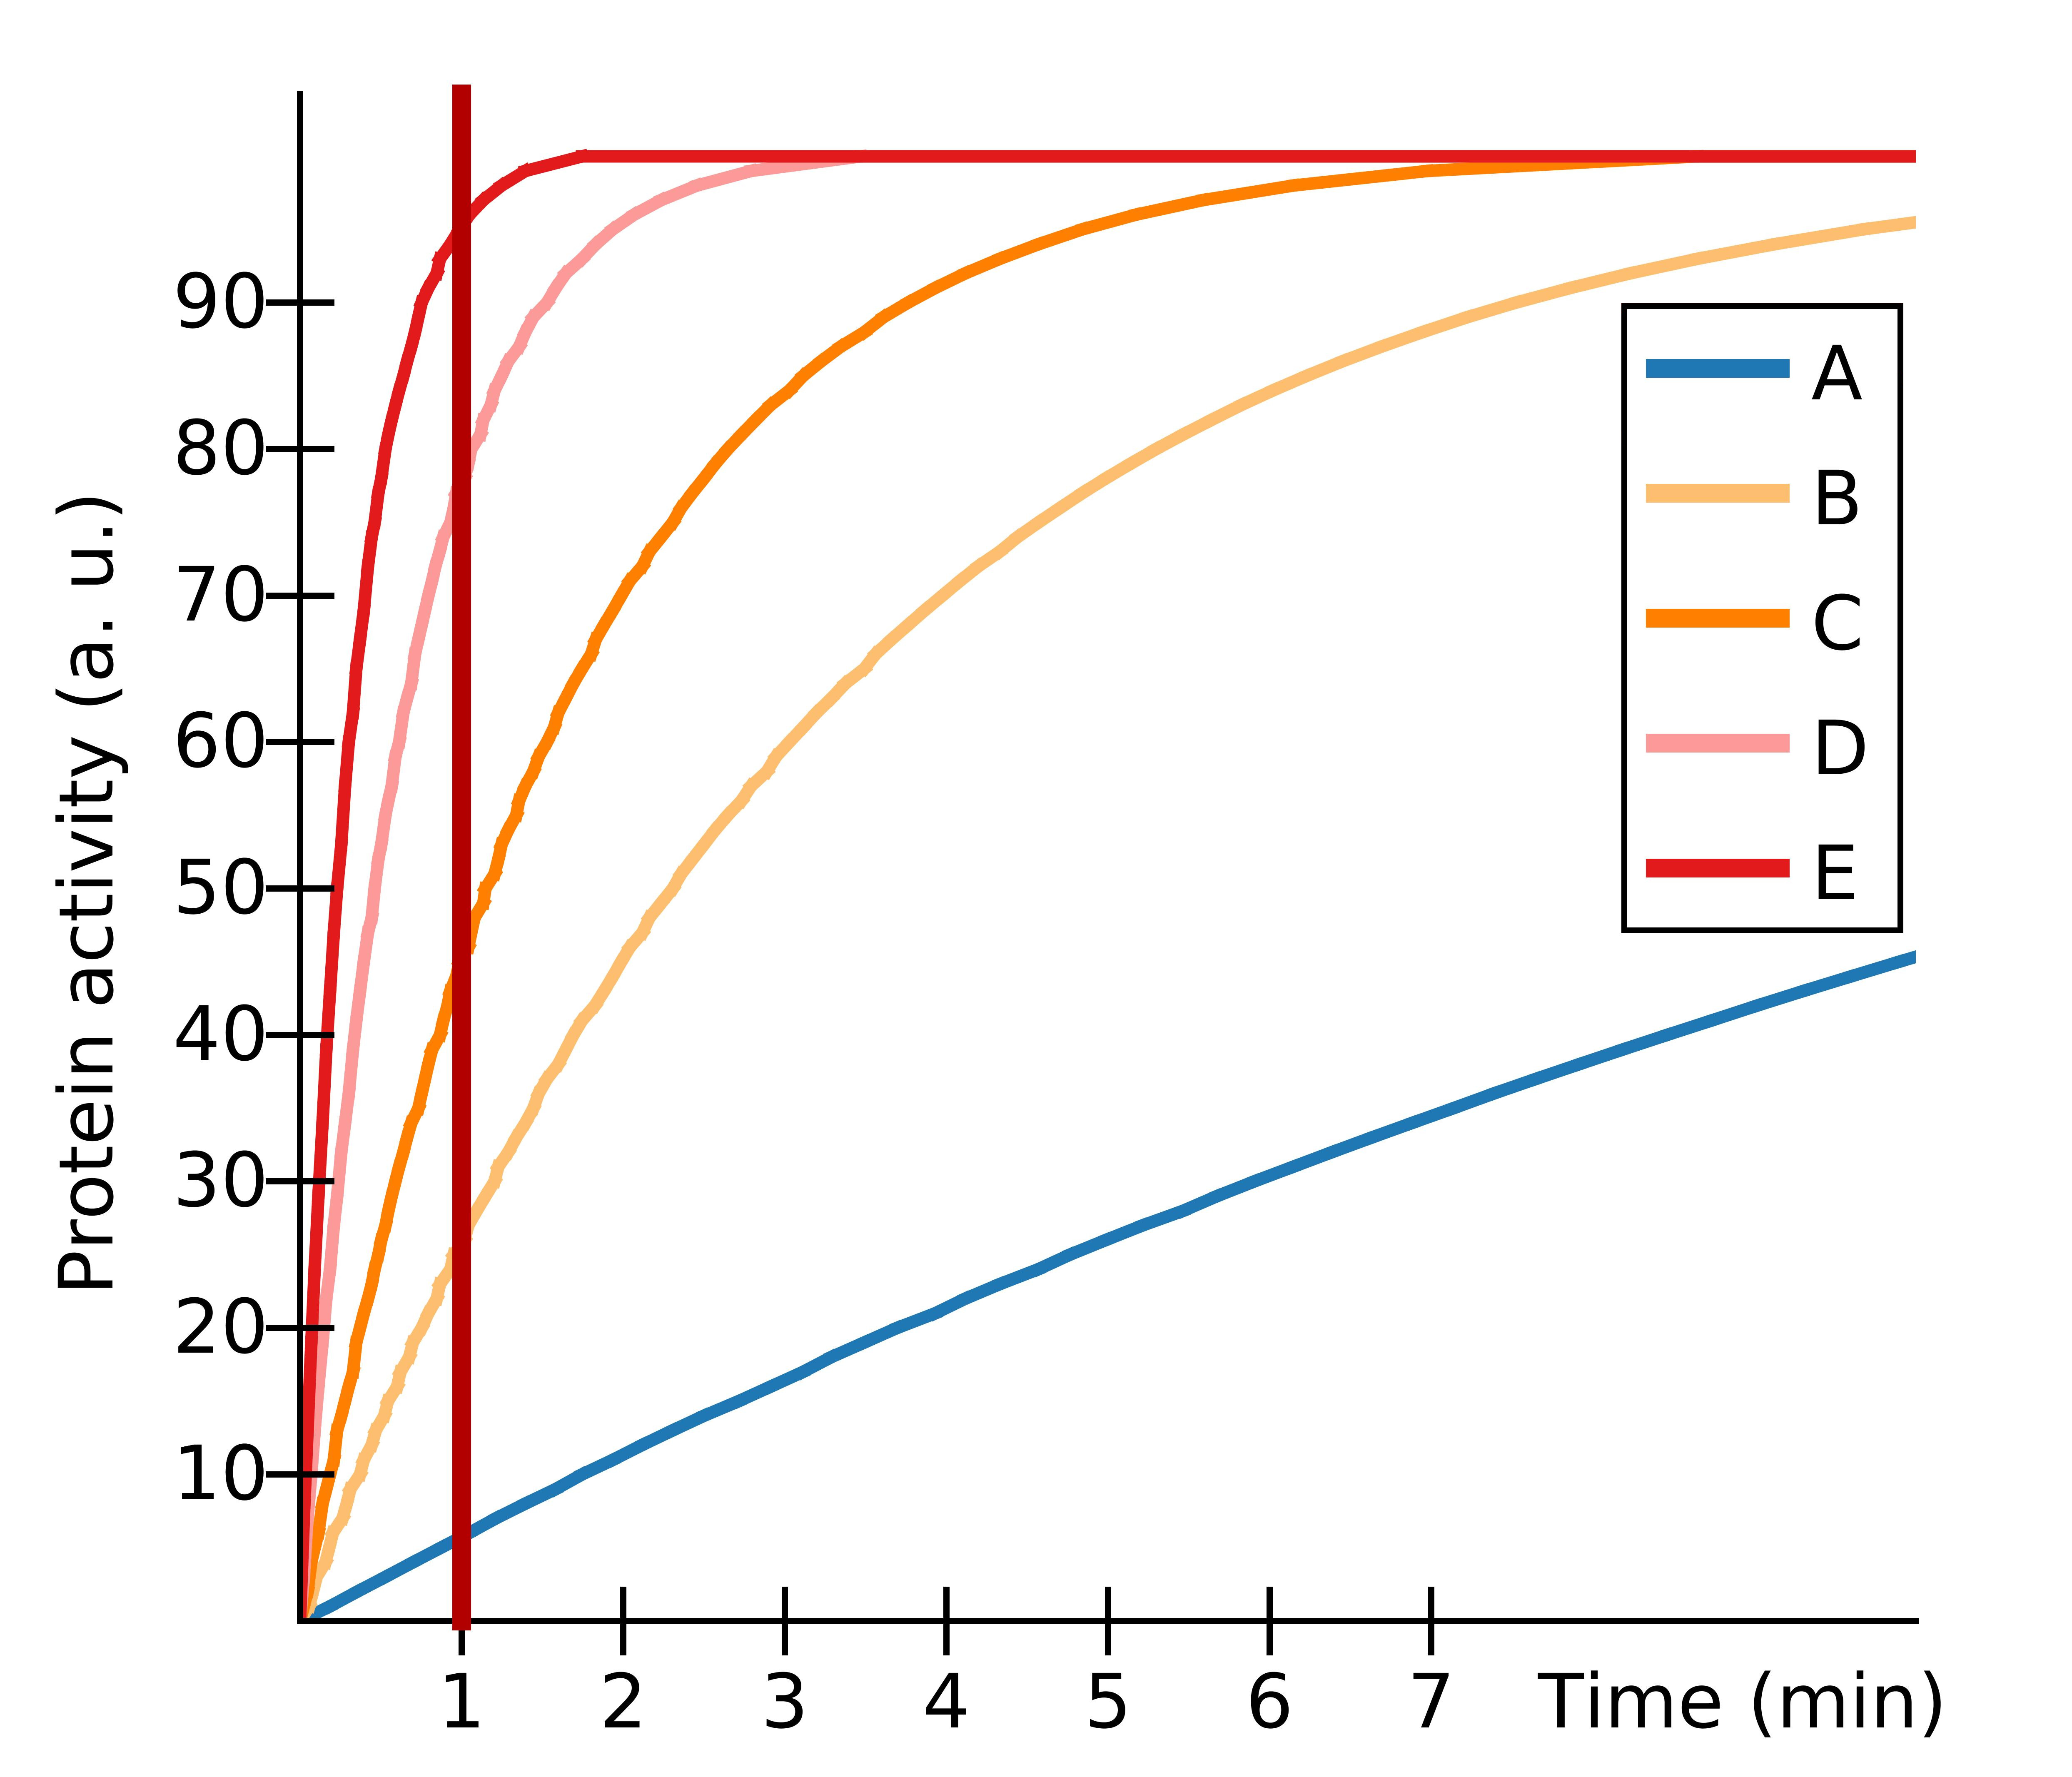
\includegraphics[scale=\graphScale]{parameter_graph}}
\end{tabular}
\caption{Example interaction settings for an ANIMO model. Each graph represents the time evolution
of the network on its left. The vertical red lines in the graphs represent the point in time on which
the coloration of the nodes in the corresponding network is based.\\
{\bf ({\protect\subref*{fig:animo-settings-scenario-network}})} The two basic scenarios. Scenario 1
makes the speed of the interaction depend only on the activity level of the upstream node {\sf Input}. In this case the
upstream node is constantly active, so the activity of {\sf A} increases linearly with time. Scenario 2
depends on the activity level of the {\sf Input} node, and on the \emph{inactivity} of {\sf B}. This
makes the rate of activation of {\sf B} decrease proportionally to the current activity level of {\sf B}:
the more {\sf B} is active, the slower the activation process will occur.\\
{\bf ({\protect\subref*{fig:animo-settings-k-network}})} Choosing a value for the scaling factor $k$. While all interactions here
are based on scenario 2, the value of their parameter $k$ (written on the edges) determines the speed at which the downstream node
is activated: a larger value of $k$ means a faster reaction.
\label{fig:animo-networks1}}
\end{figure*}


\begin{figure*}[htbp]
\centering
\begin{tabular}{ll}
\subfloat[\label{fig:animo-settings-direct-network}]{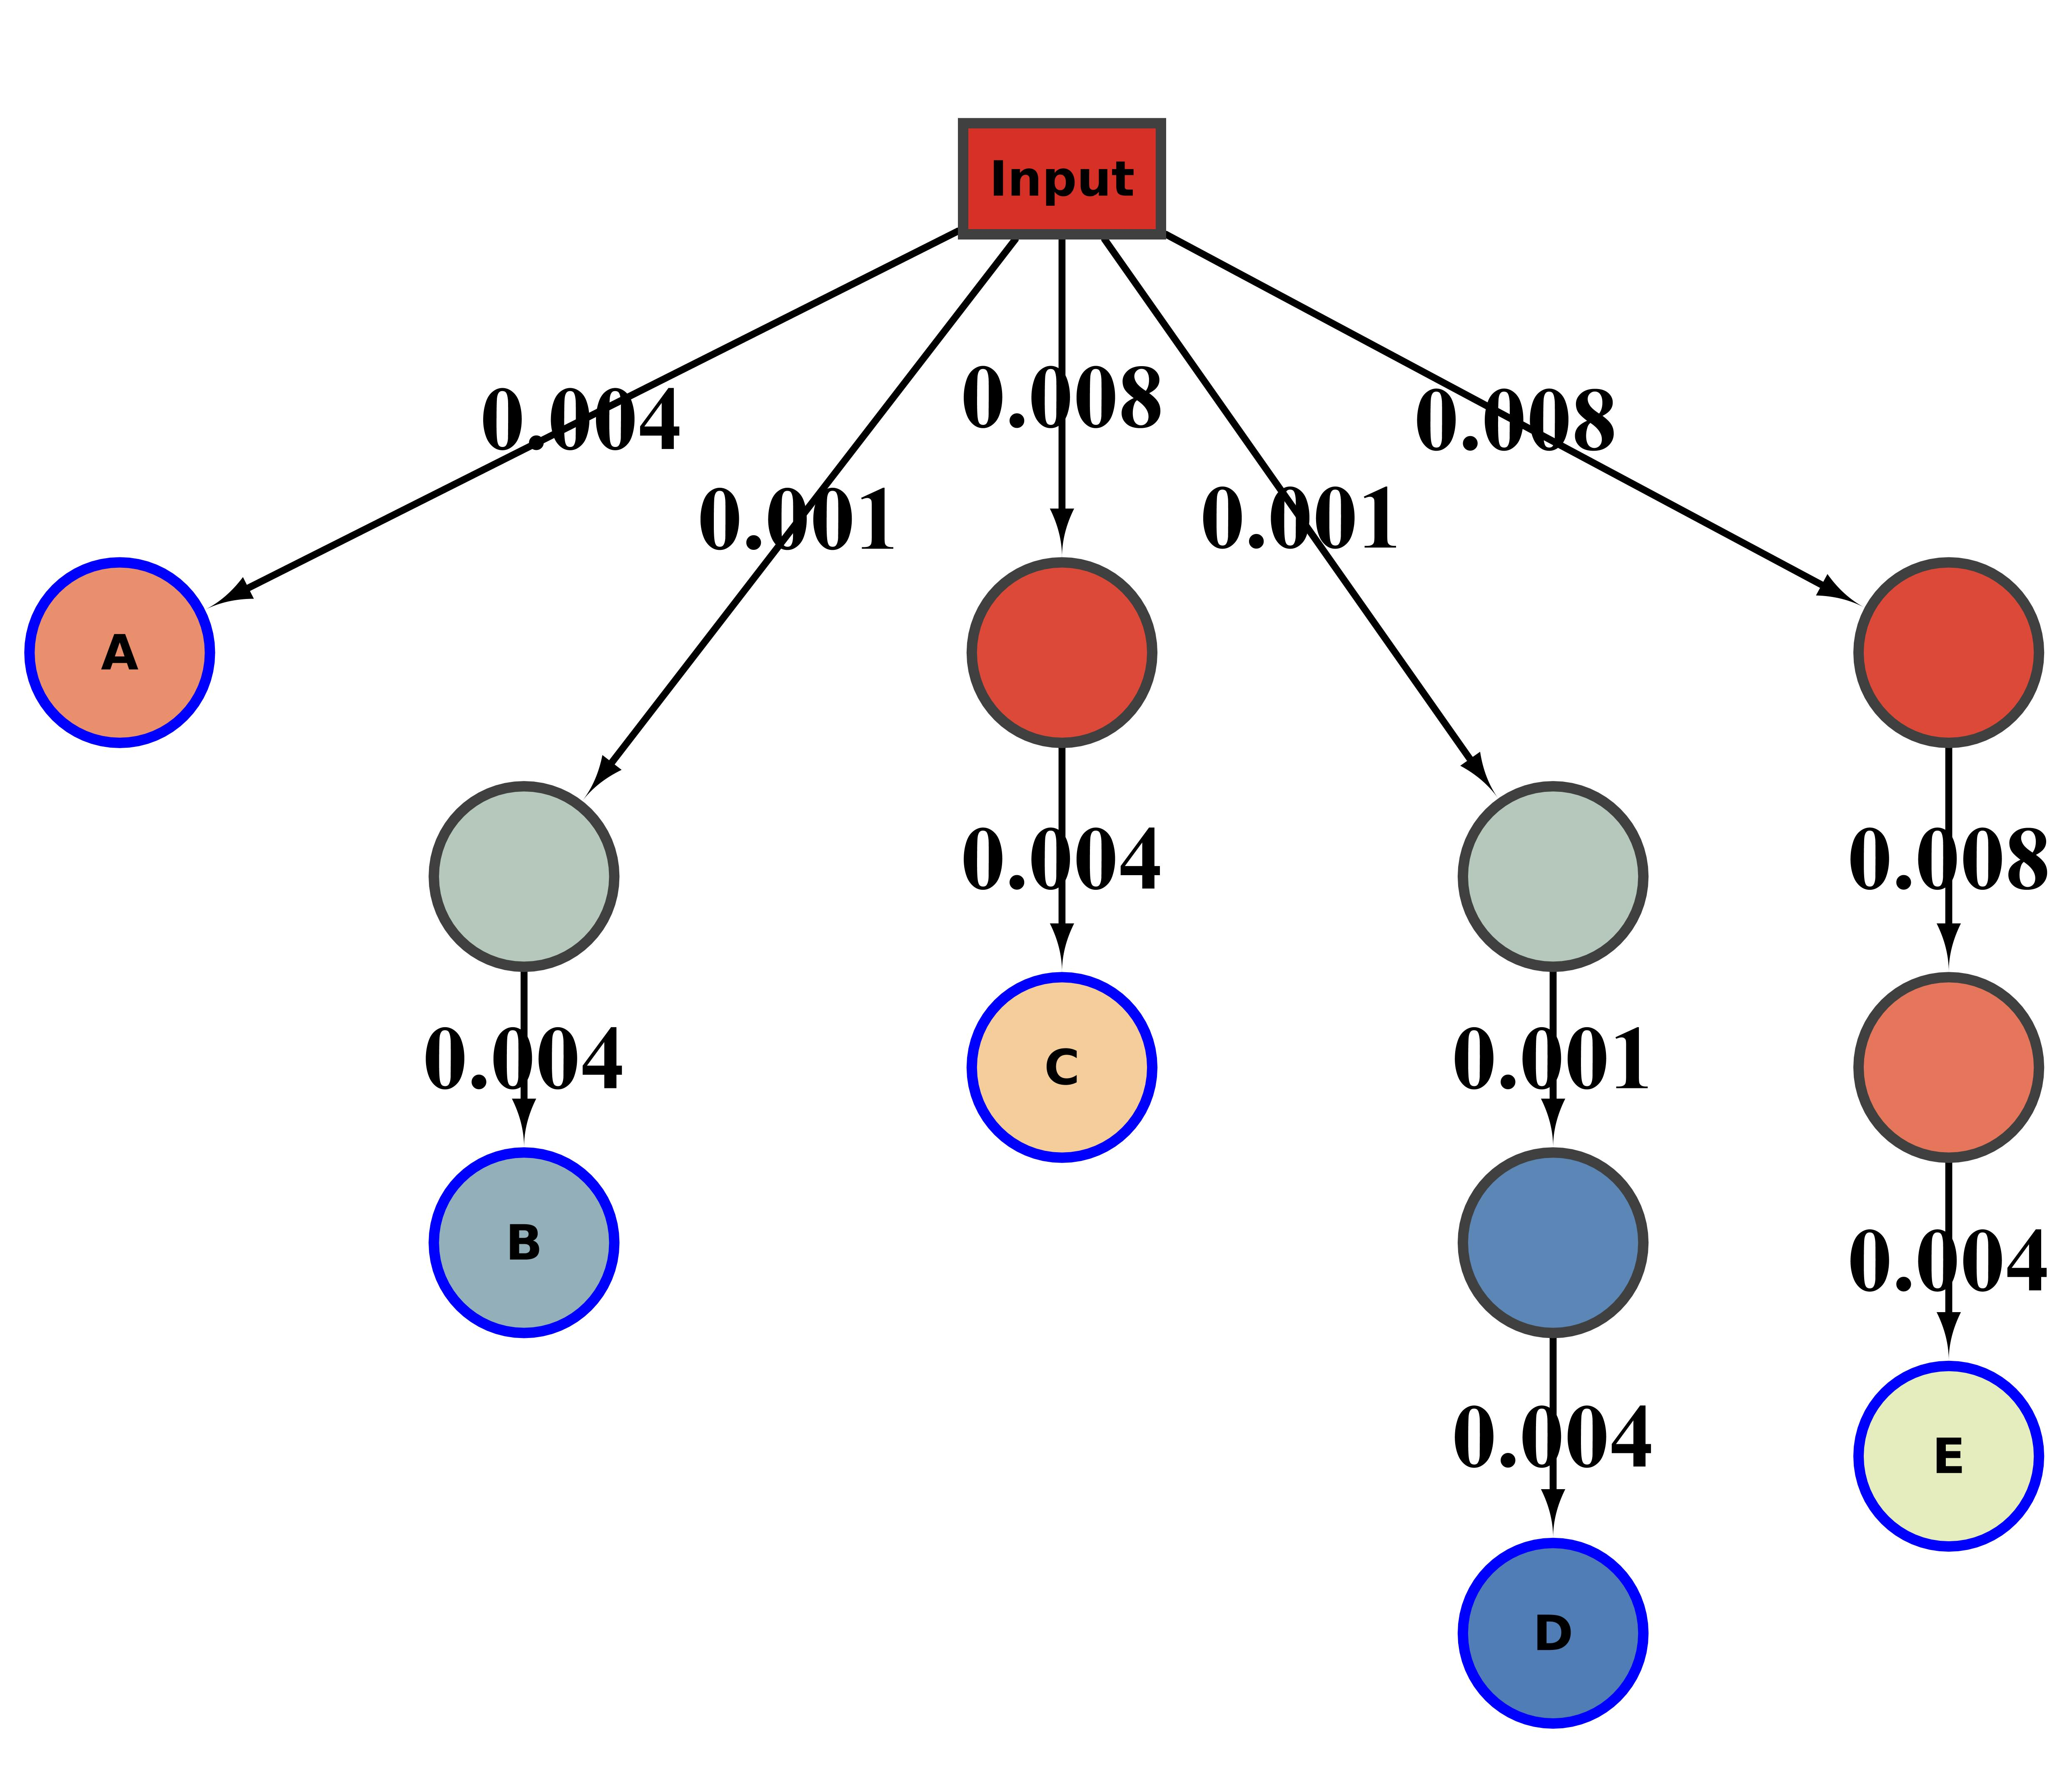
\includegraphics[scale=\graphScale]{direct_indirect_network_CB}} & 
\subfloat[\label{fig:animo-settings-direct-graph}]{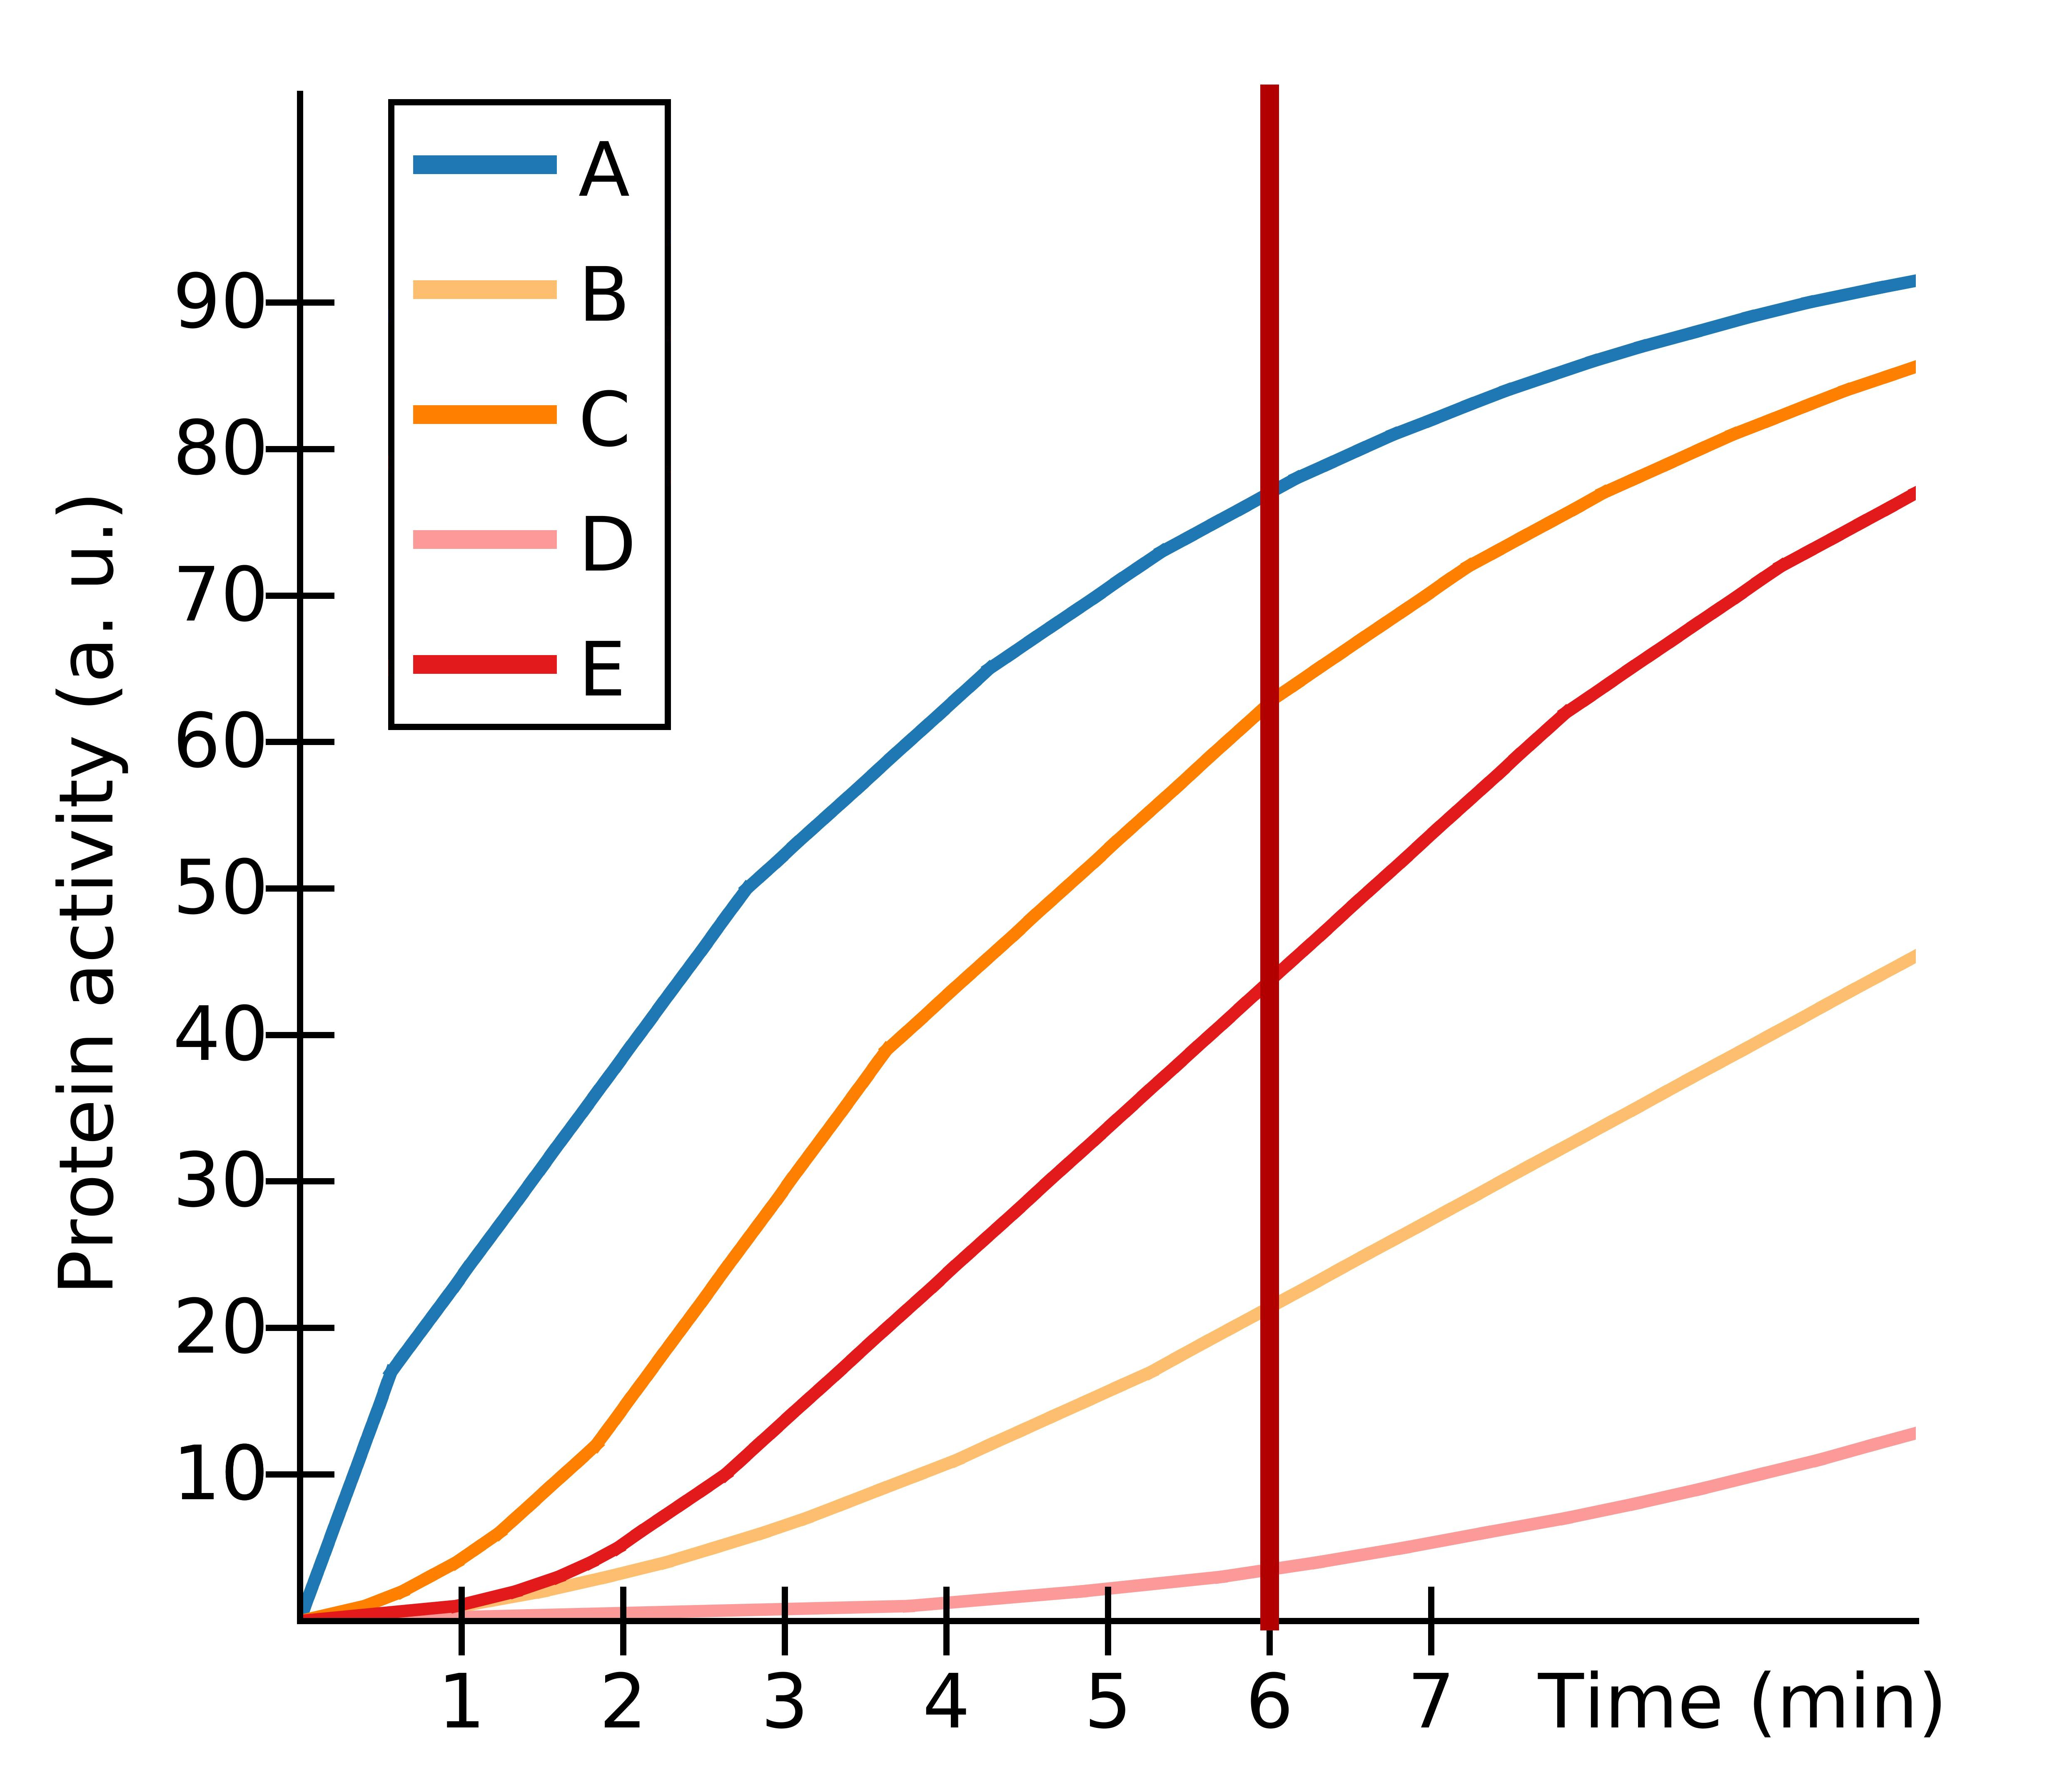
\includegraphics[scale=\graphScale]{direct_indirect_graph}} \\ 
\subfloat[\label{fig:animo-settings-feedback-network}]{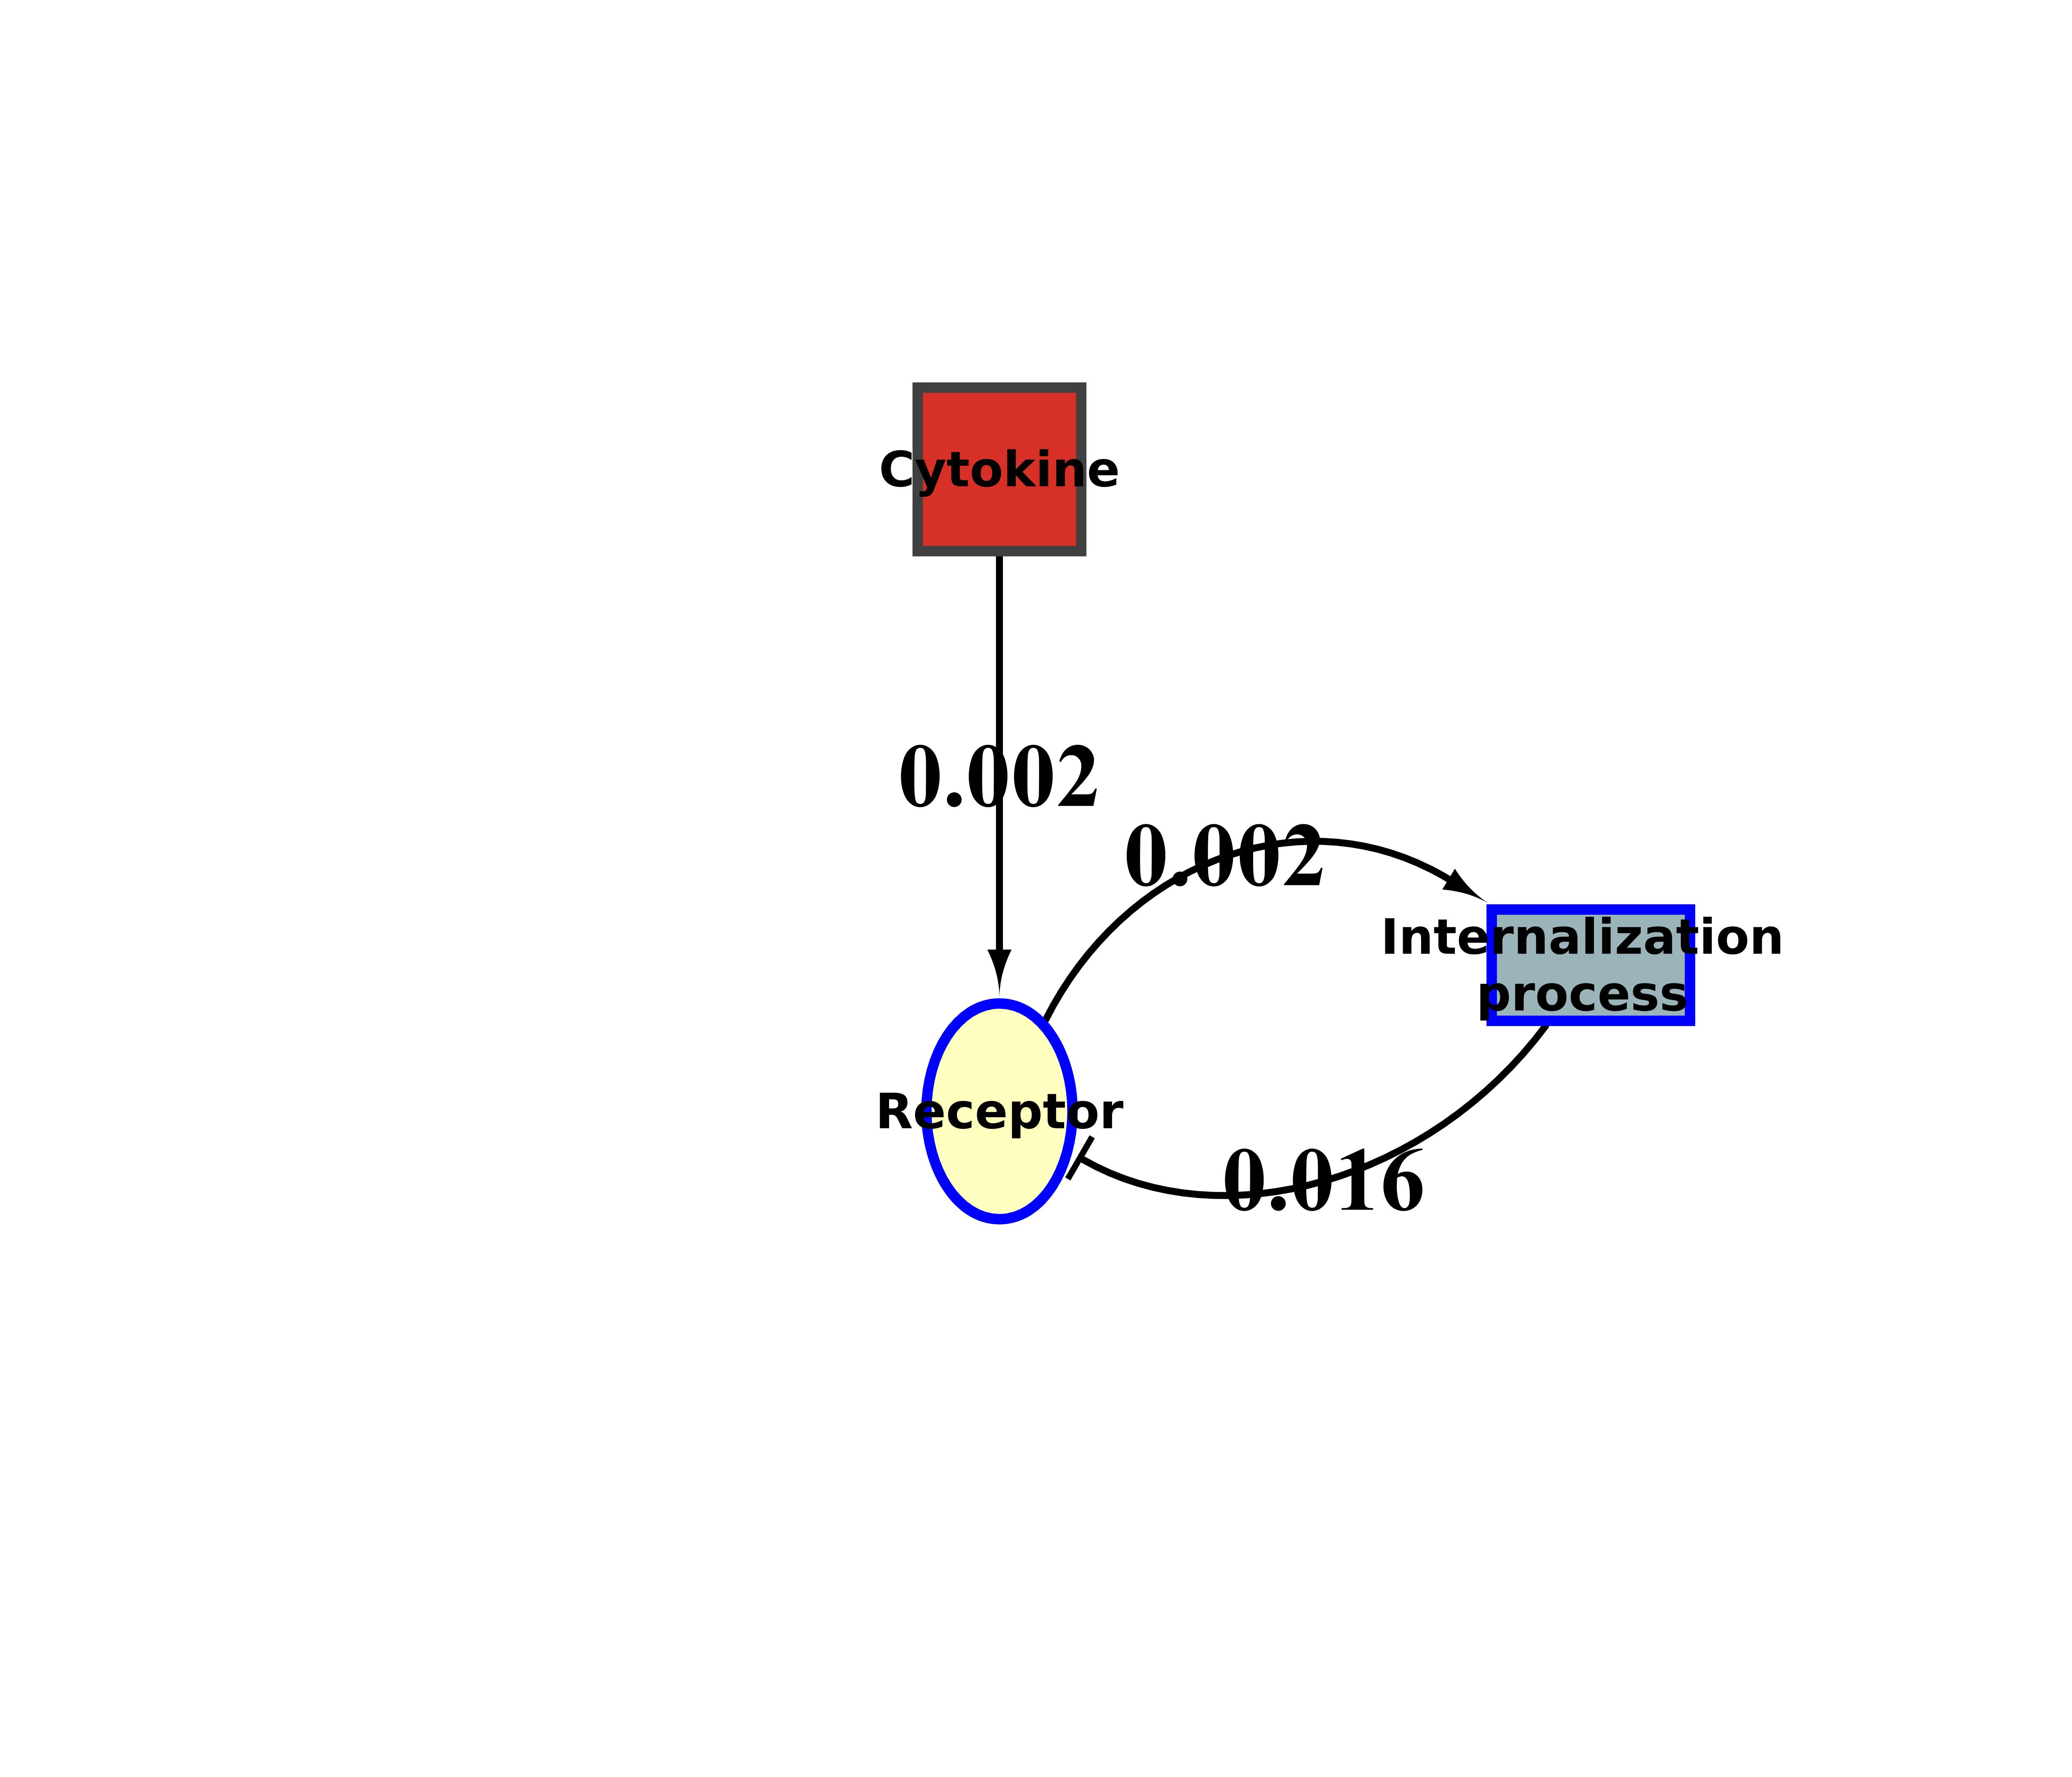
\includegraphics[scale=\graphScale]{feedback_network_CB}} & 
\subfloat[\label{fig:animo-settings-feedback-graph}]{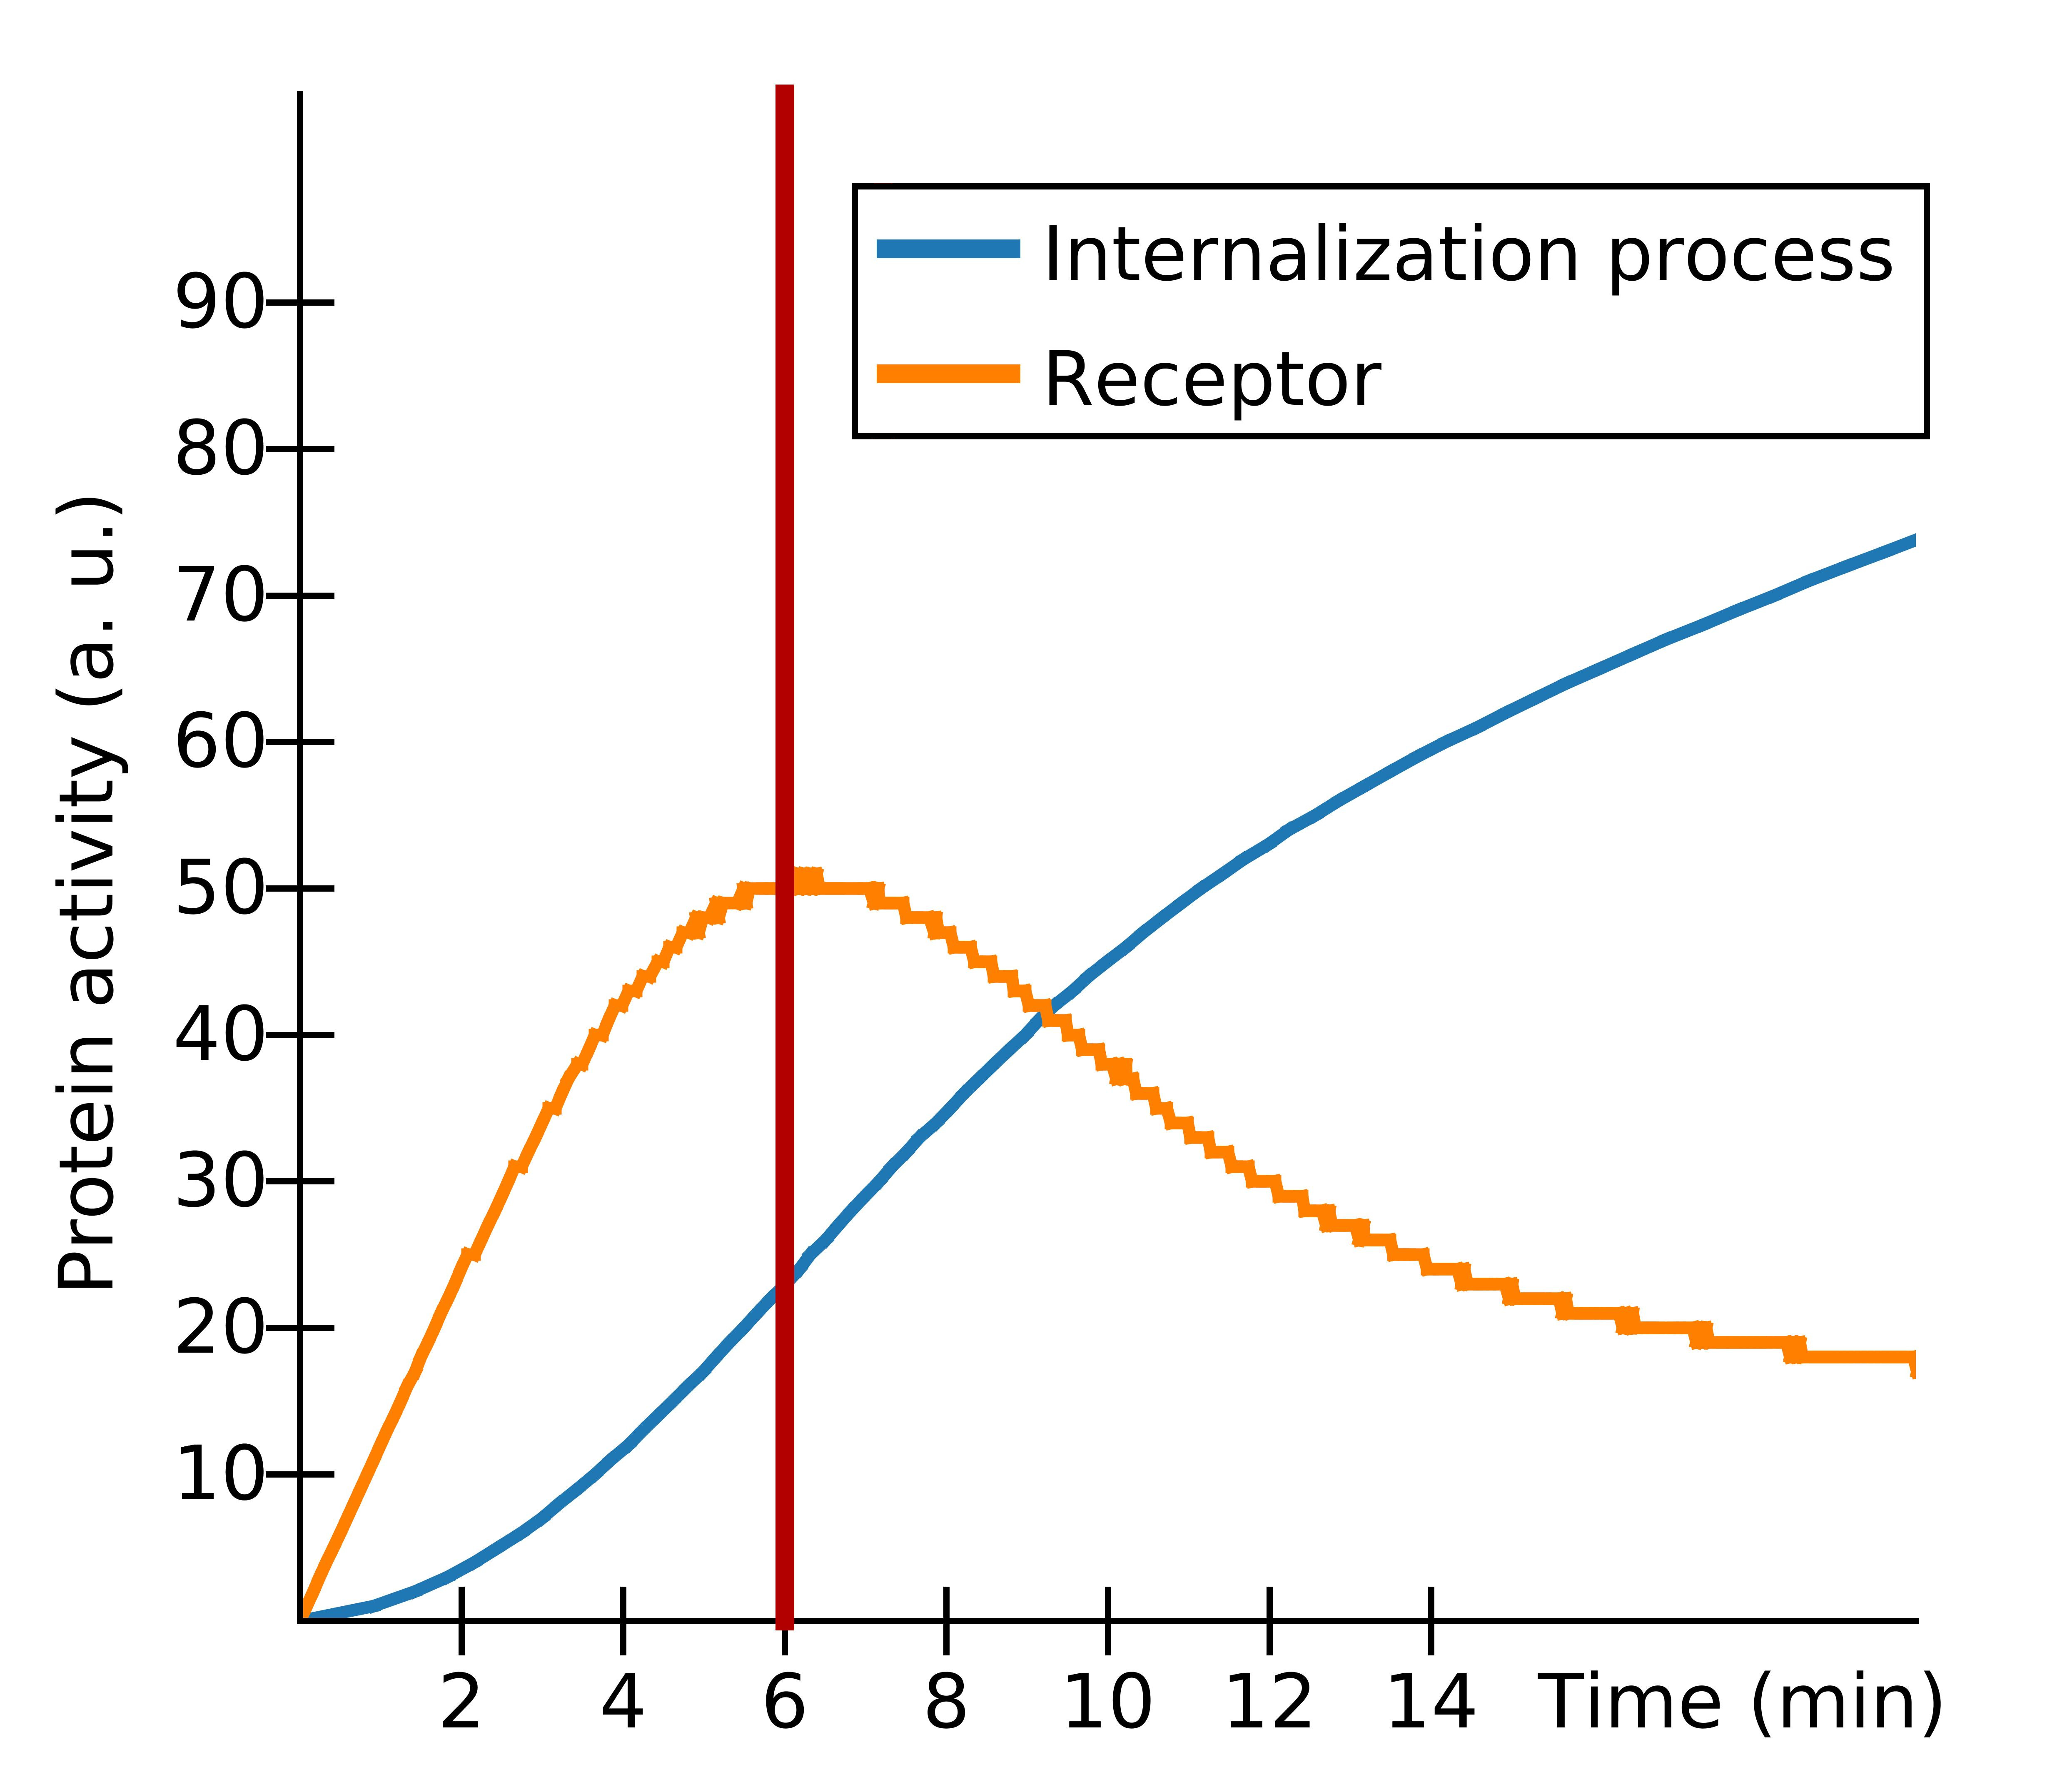
\includegraphics[scale=\graphScale]{feedback_graph}}
\end{tabular}
\caption{Example interaction settings for an ANIMO model. Each graph represents the time evolution
of the network on its left. The vertical red lines in the graphs represent the point in time on which
the coloration of the nodes in the corresponding network is based.\\
{\bf ({\protect\subref*{fig:animo-settings-direct-network}})} Relation between network topology and delays. In order to delay the activation process
ensuing an external signal (node {\sf Input}), we can reduce the reaction speed by changing $k$ or
adding an intermediate node. Introducing a slowly activated ($k = 0.001$) node between {\sf Input} and {\sf B} is enough to
activate {\sf B} at a much slower rate than {\sf A}, even if the value of $k$ for the last step is left unchanged at $k = 0.004$.
Increasing the parameter of the newly introduced reaction lets us fine tune
the speed of the response, making the activation of {\sf C} faster than {\sf B}, but still slower than {\sf A}. We repeat the process
of introducing a delay with nodes {\sf D} and {\sf E}: an additional intermediate node further reduces the response time.\\
{\bf ({\protect\subref*{fig:animo-settings-feedback-network}})} Peak dynamics are often observed in experimental data.
In order to have the activity level of a node increase and successively decrease, the simplest way is to model it with a feed-back loop.
In the example, we model the internalization of a receptor following its activation. Note that the interaction {\sf Internalization
process} $\dashv$ {\sf Receptor} is an inhibition: being based on scenario 2, it will reduce the activity of the {\sf Receptor} node with a rate proportional
to the current activity of both involved nodes. Scenario 1 dynamics are sufficient to model the two activating reactions {\sf Cytokine} $\rightarrow$ {\sf Receptor}
and {\sf Receptor} $\rightarrow$ {\sf Internalization Process}. Key to the peak dynamics is the fact that the inactivation of the {\sf Receptor} node
is much faster (higher $k$ value) than its activation.
\label{fig:animo-networks2}}
\end{figure*}

%Full figure in one page:
% \def\graphScale{0.0243}
% \begin{figure*}[htbp]
% \centering
% \begin{tabular}{llll}
% \subfloat[\label{fig:animo-settings-scenario-network}]{\includegraphics[scale=\graphScale]{scenario1-2_network_legend_CB}} &
% \subfloat[\label{fig:animo-settings-scenario-graph}]{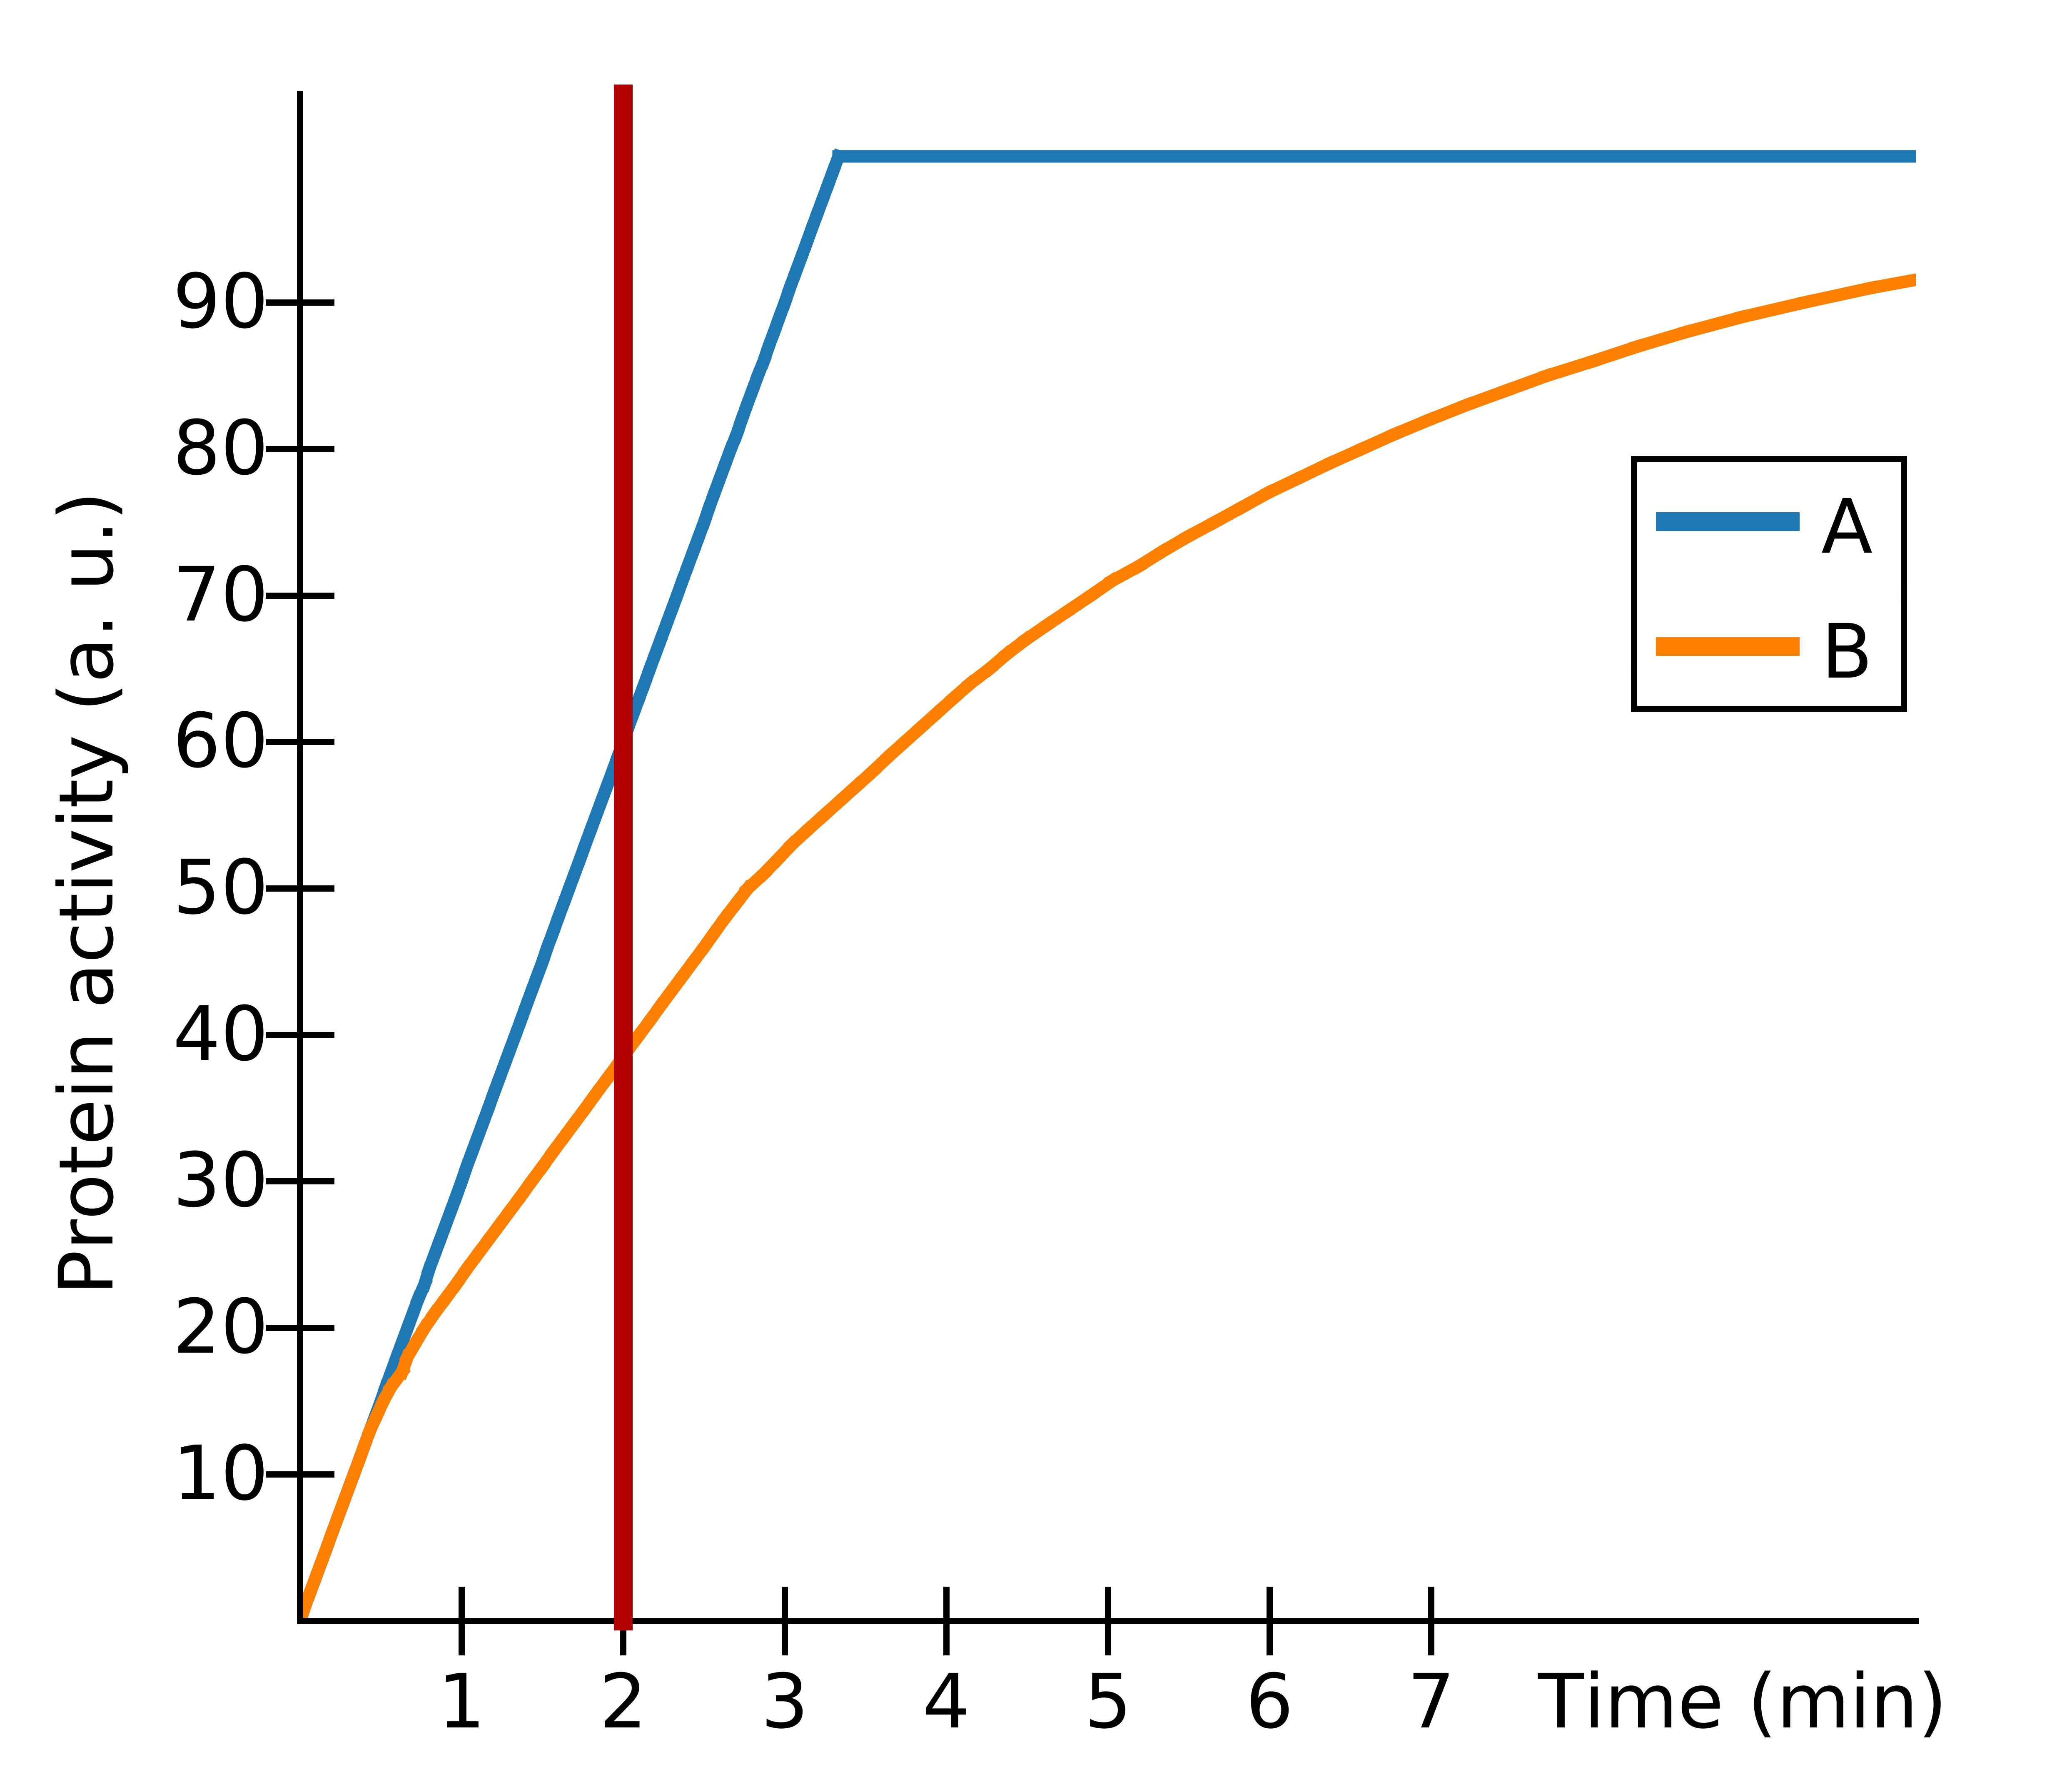
\includegraphics[scale=\graphScale]{scenario1-2_graph}} &
% \subfloat[\label{fig:animo-settings-k-network}]{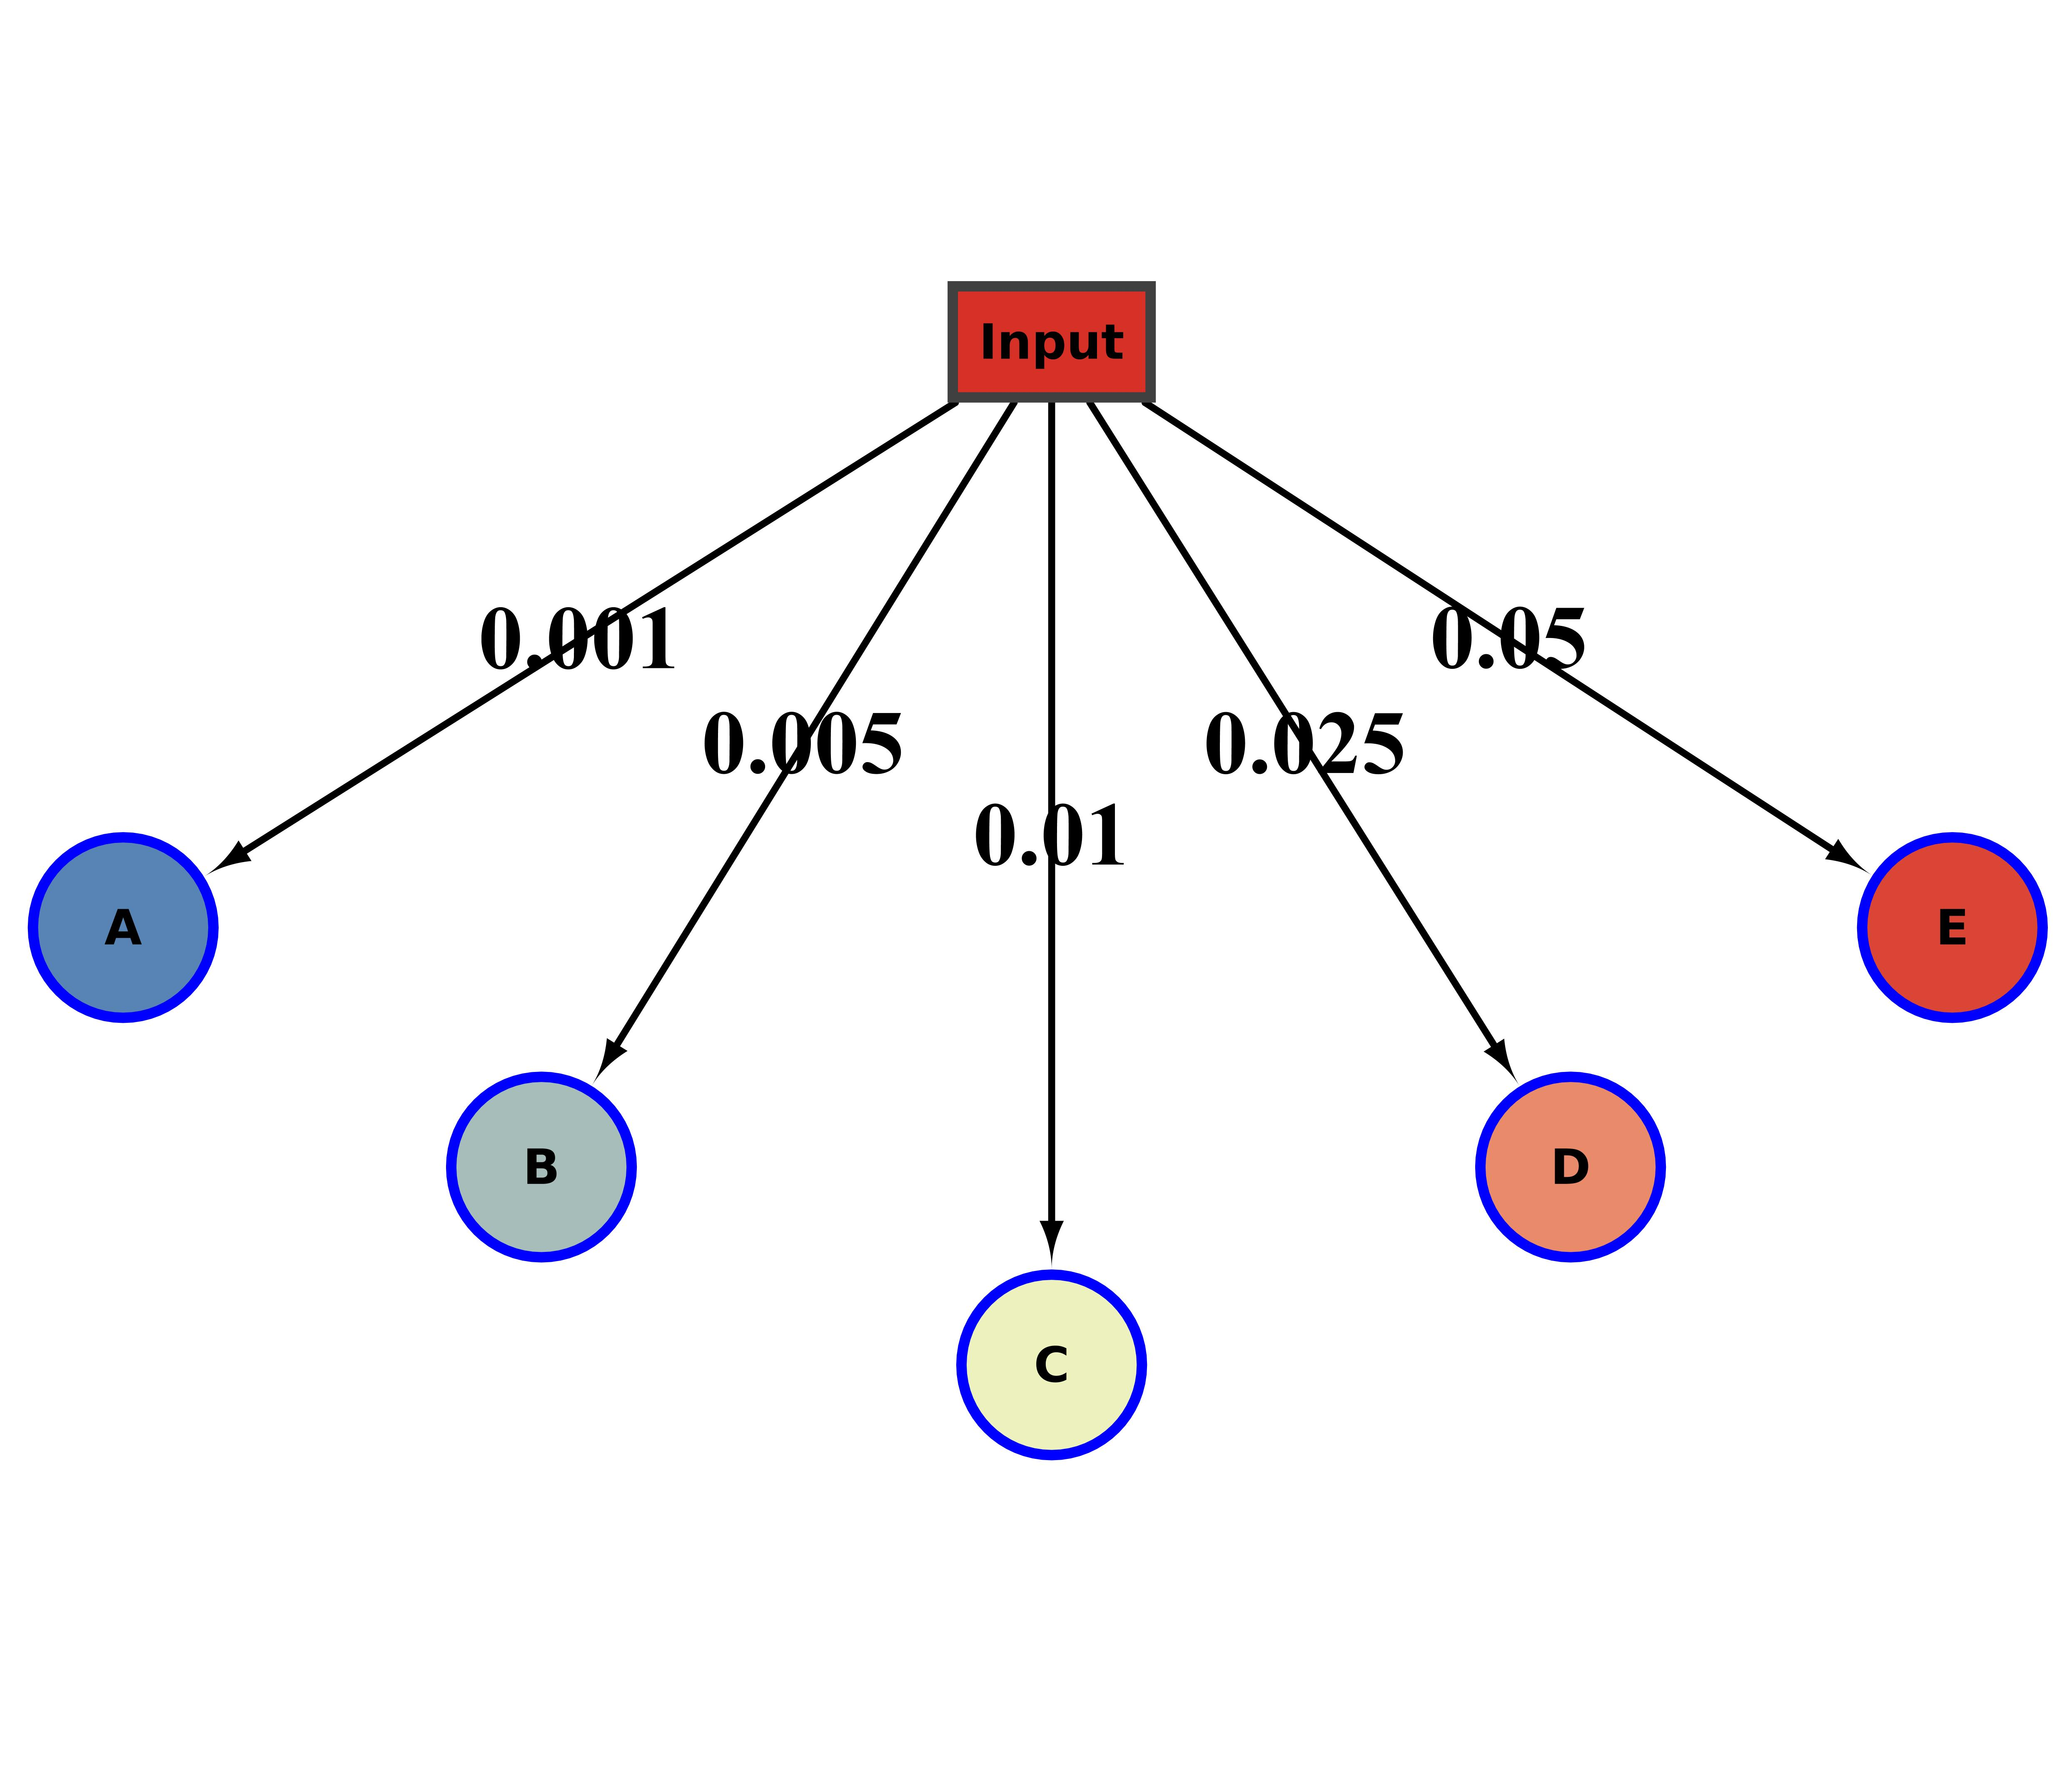
\includegraphics[scale=\graphScale]{parameter_network_CB}} &
% \subfloat[\label{fig:animo-settings-k-graph}]{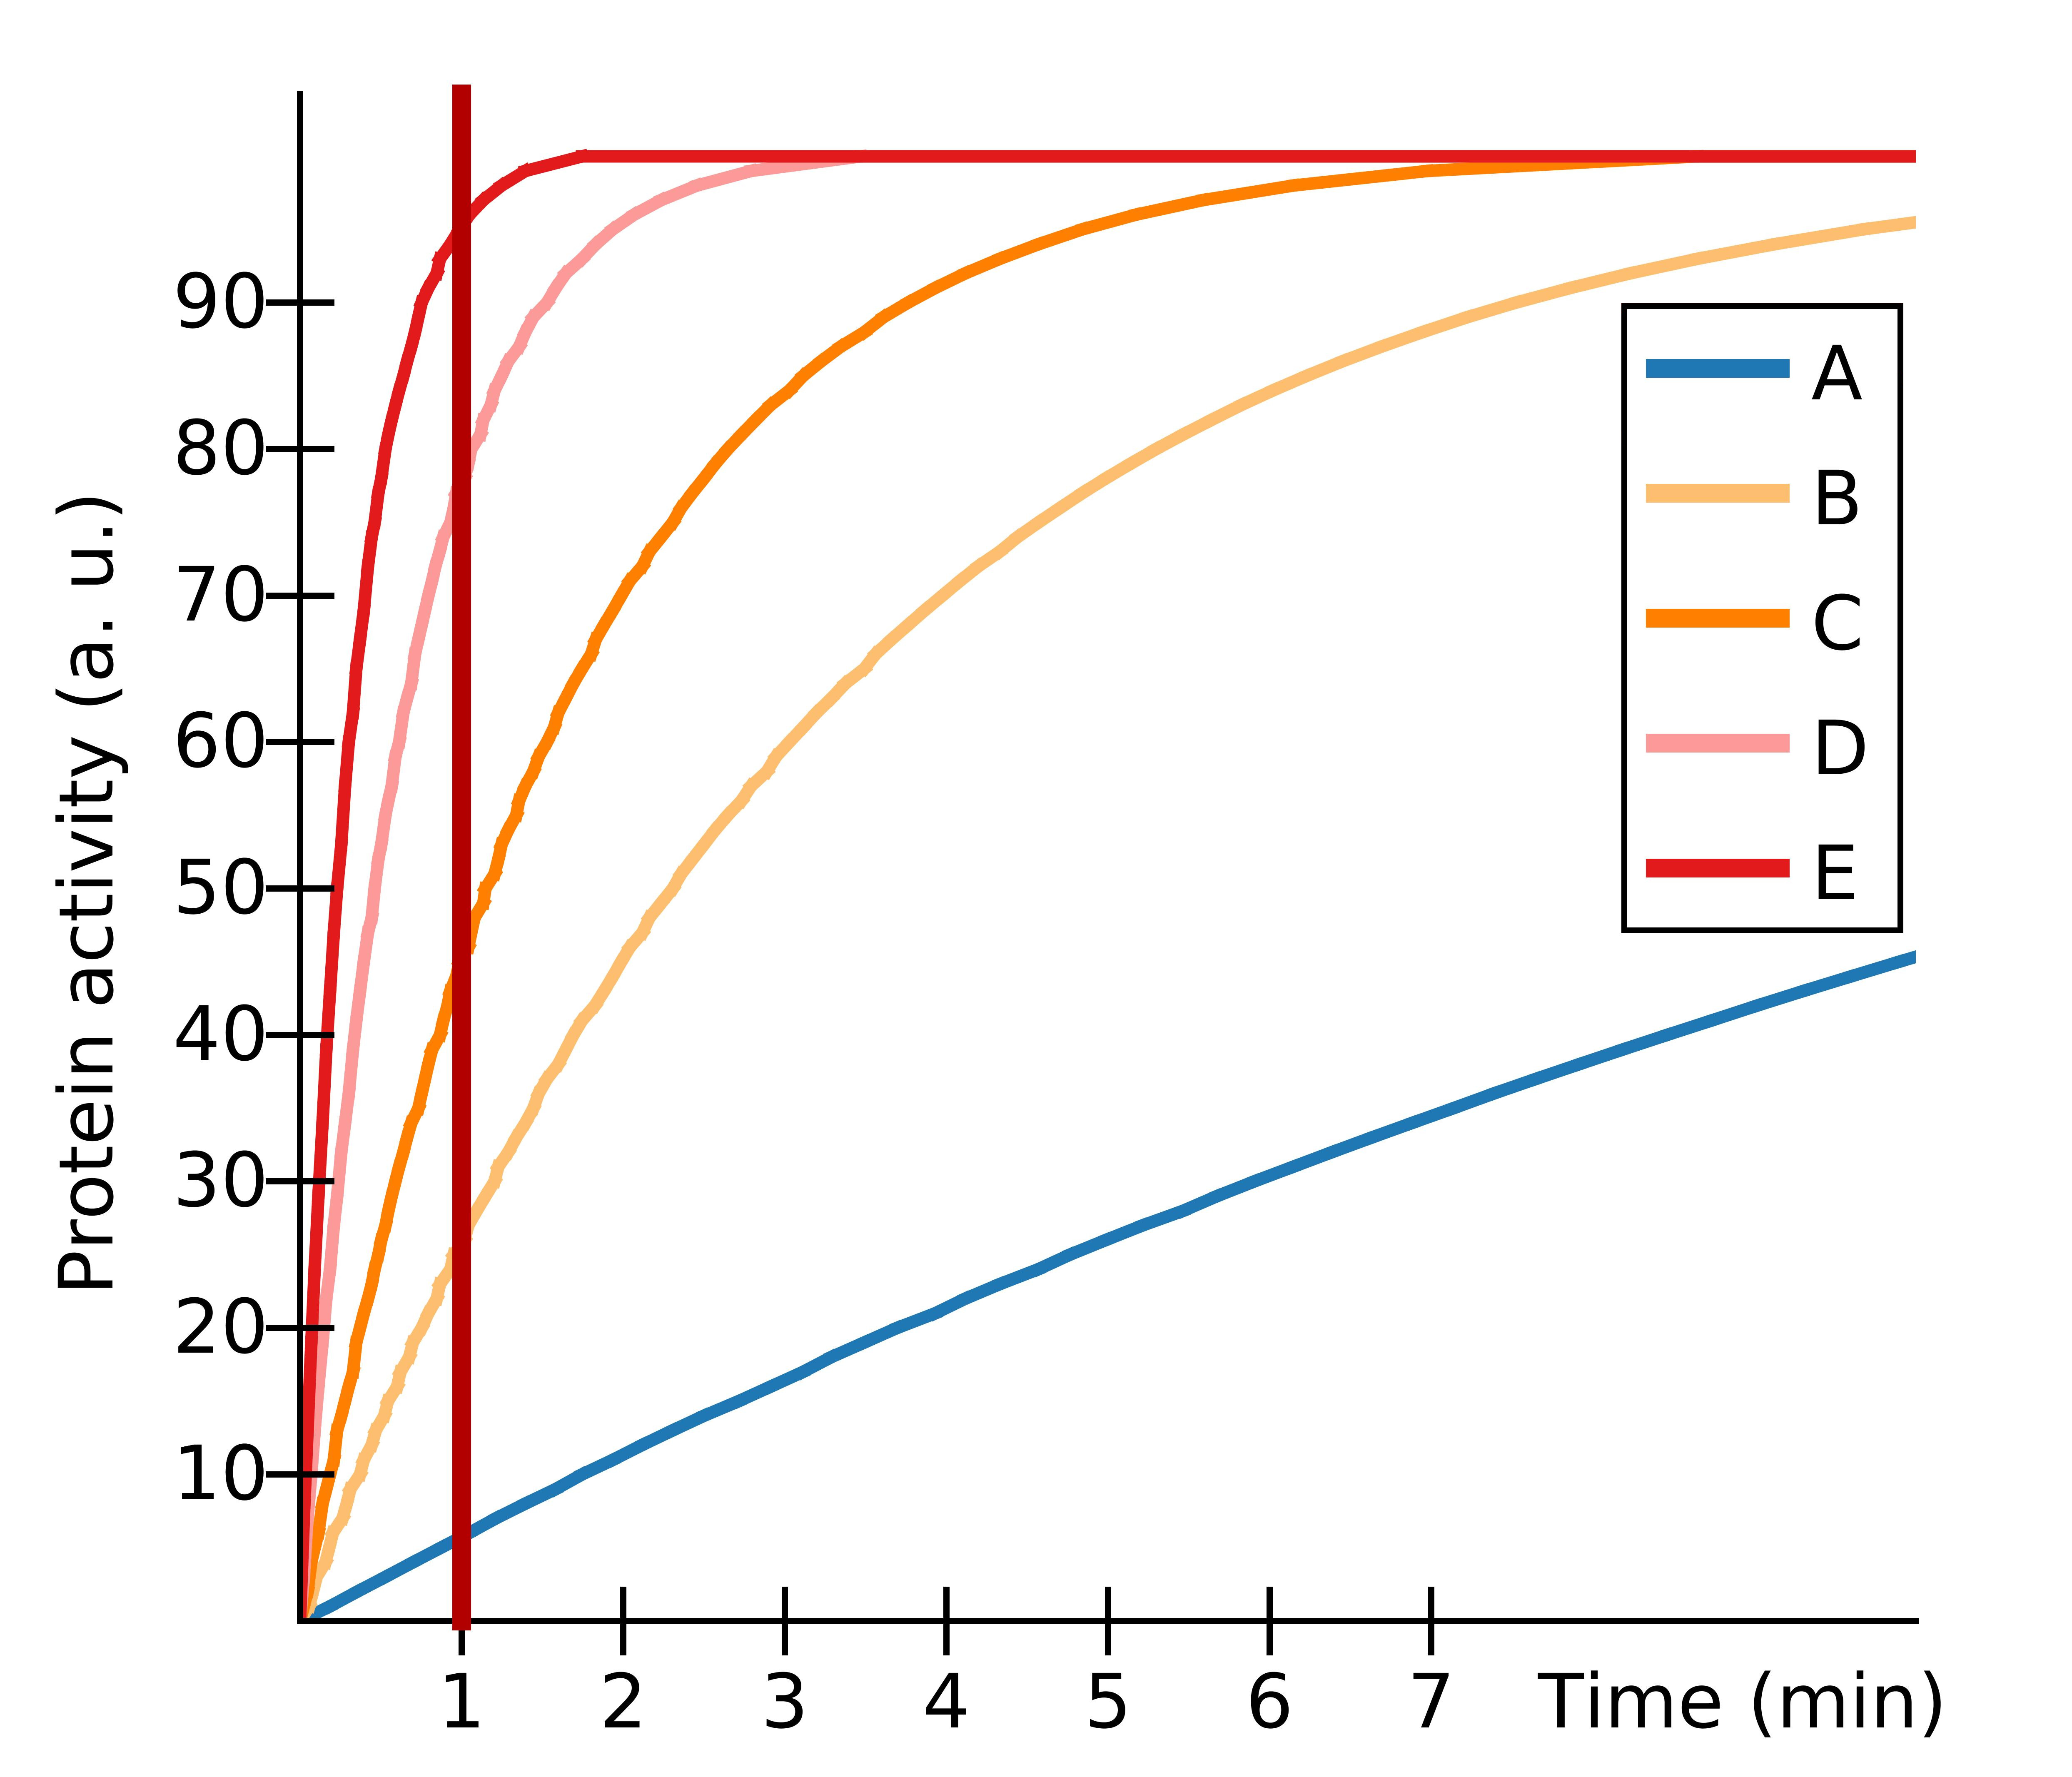
\includegraphics[scale=\graphScale]{parameter_graph}} \\
% \subfloat[\label{fig:animo-settings-direct-network}]{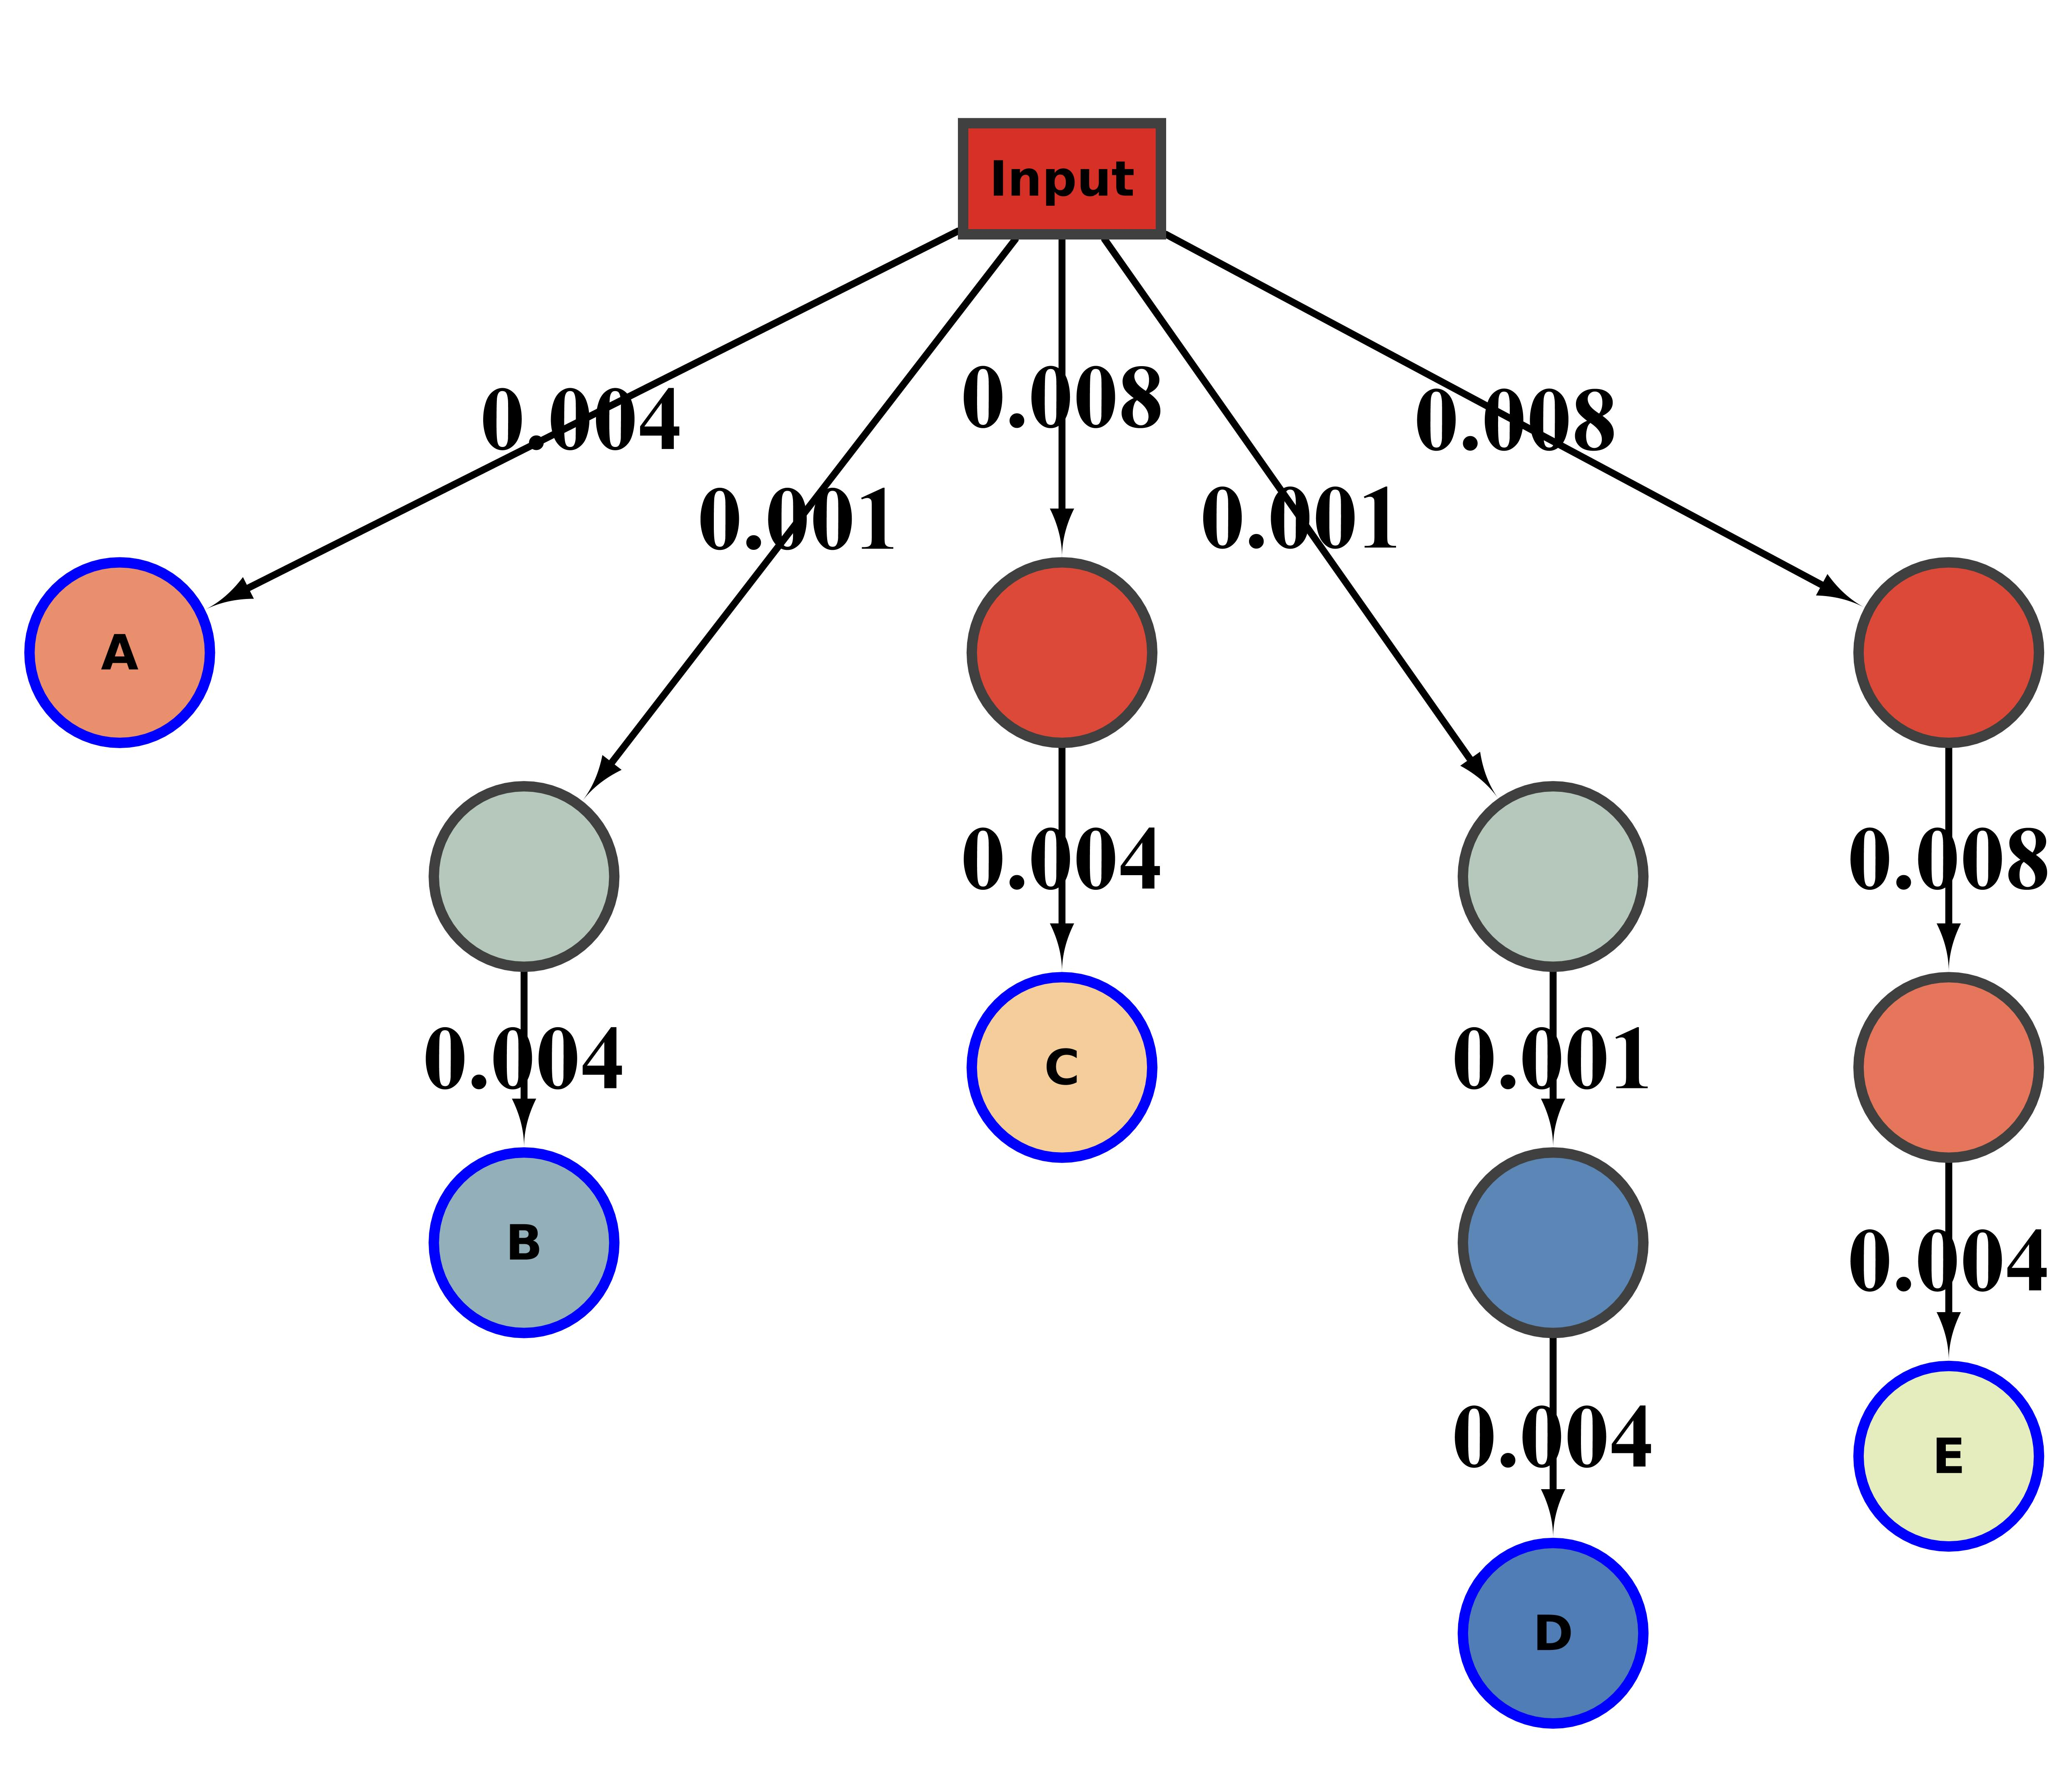
\includegraphics[scale=\graphScale]{direct_indirect_network_CB}} & 
% \subfloat[\label{fig:animo-settings-direct-graph}]{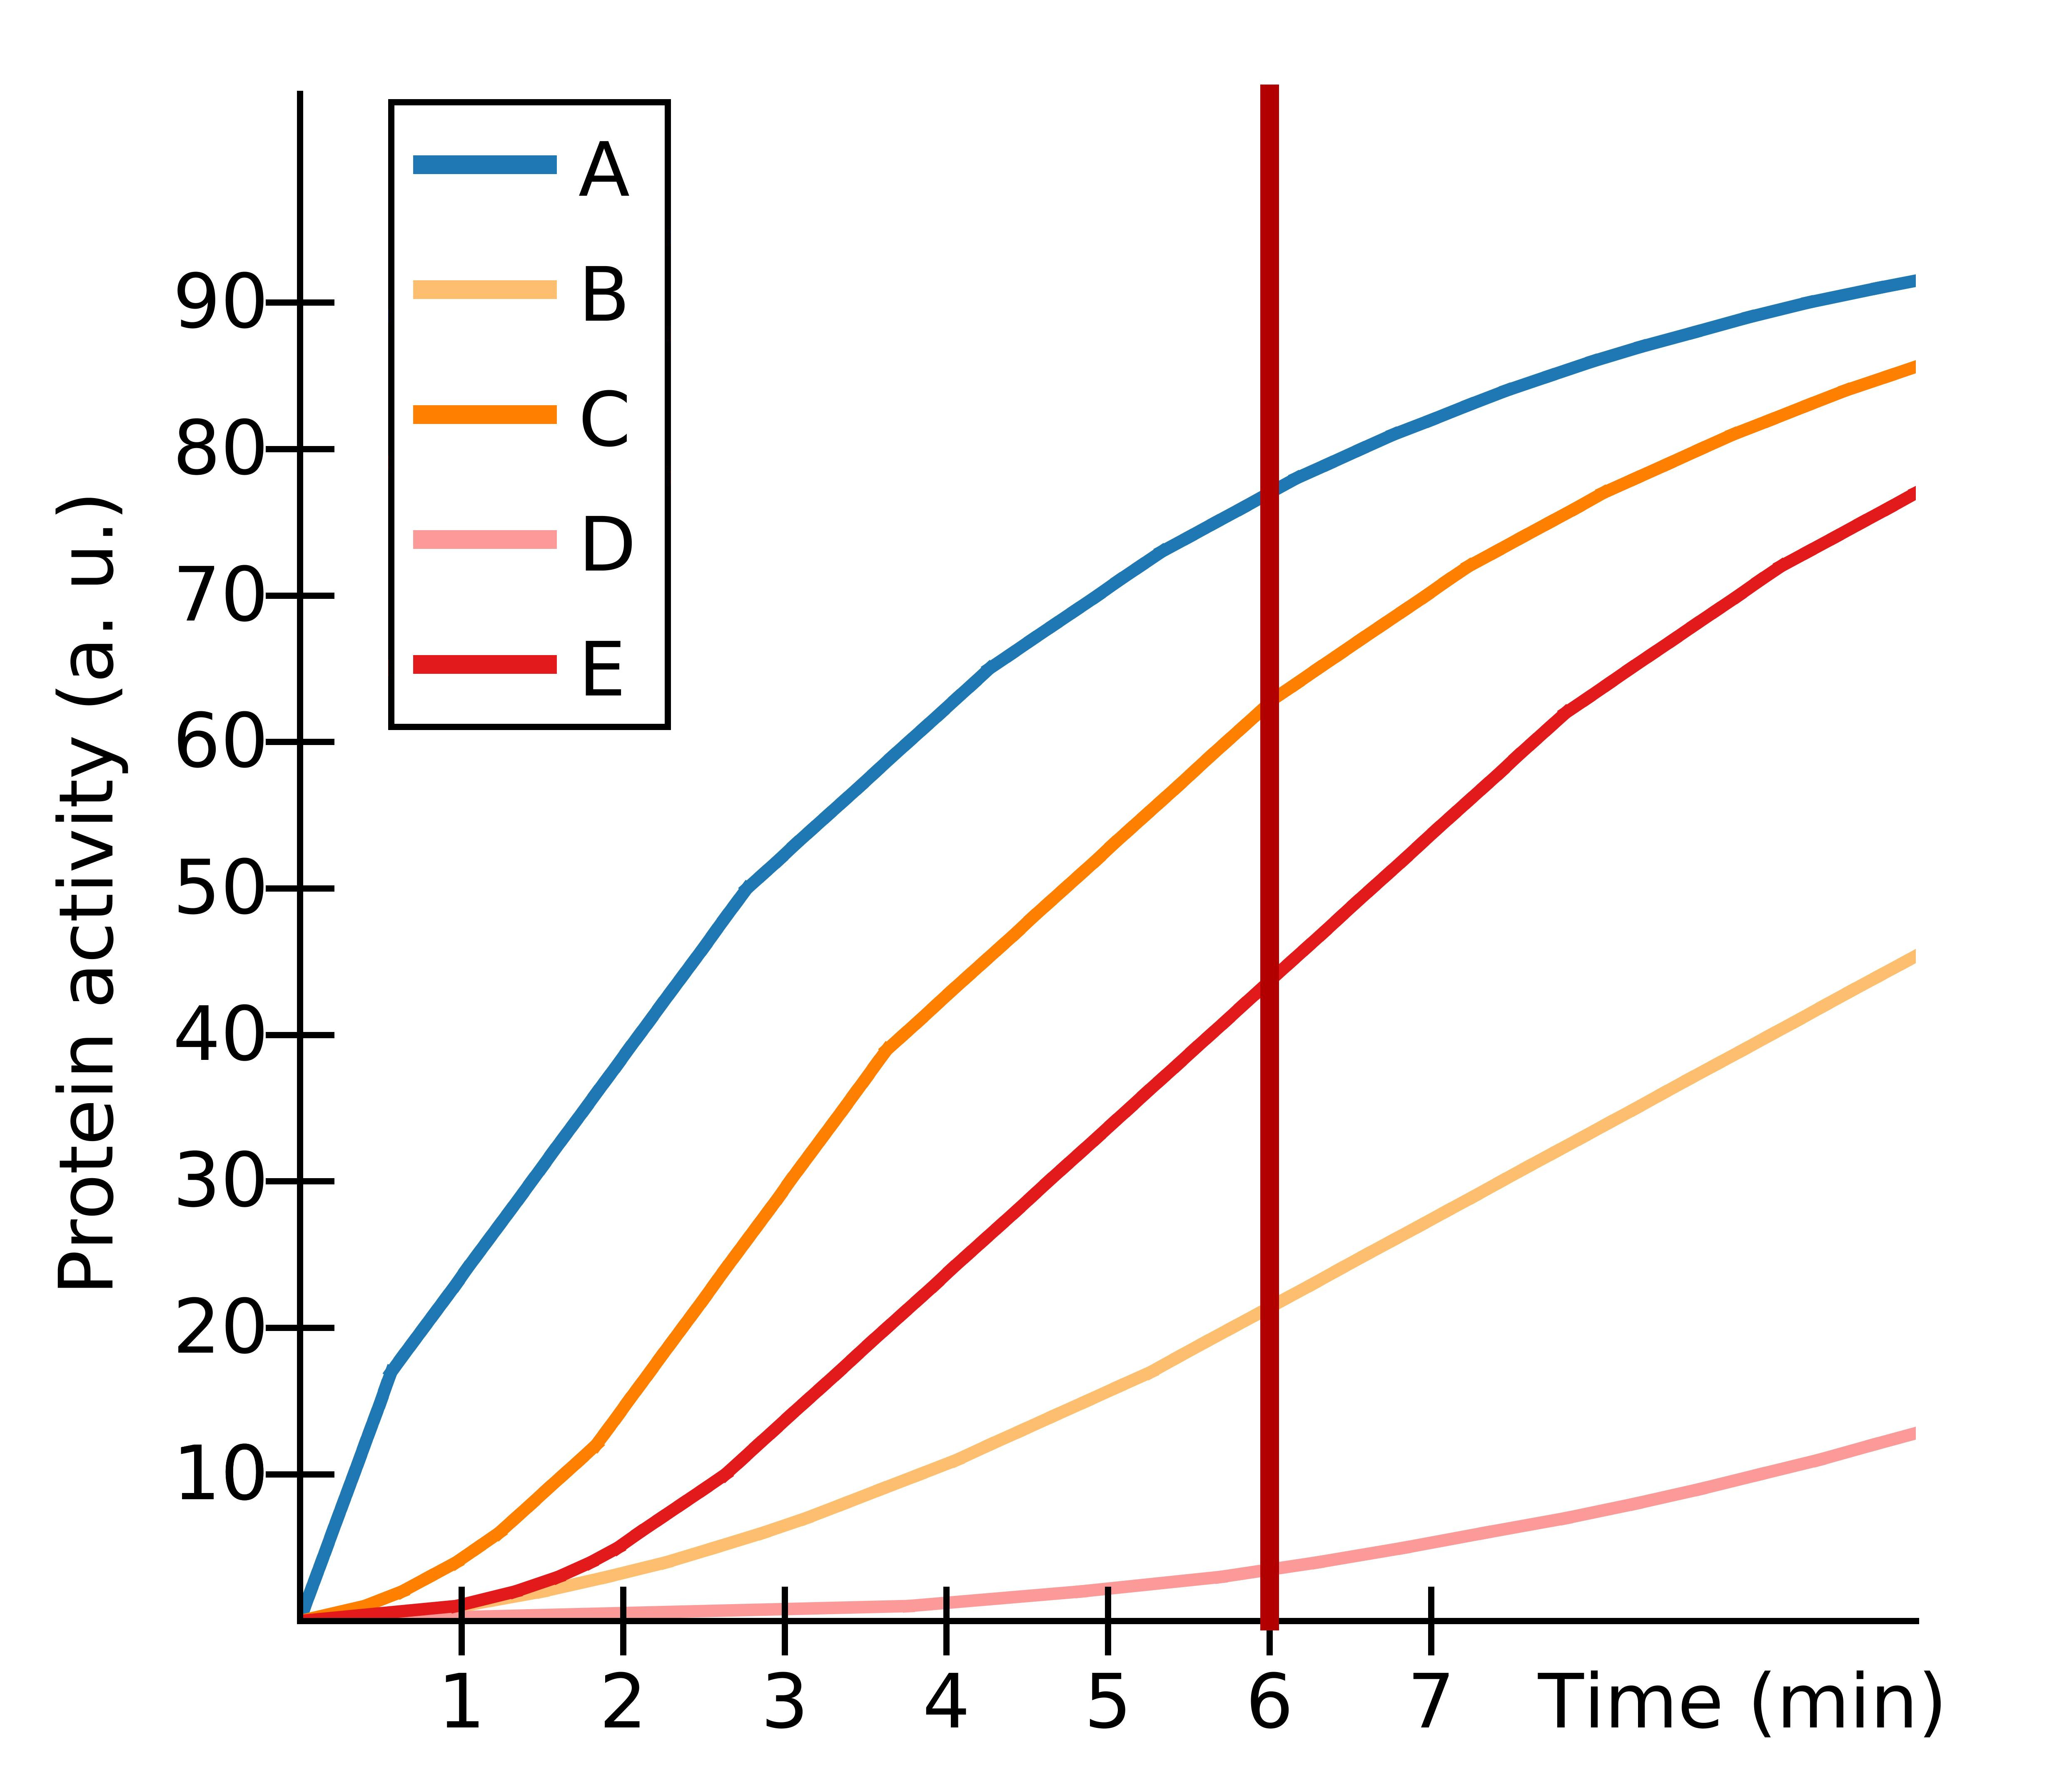
\includegraphics[scale=\graphScale]{direct_indirect_graph}} & 
% \subfloat[\label{fig:animo-settings-feedback-network}]{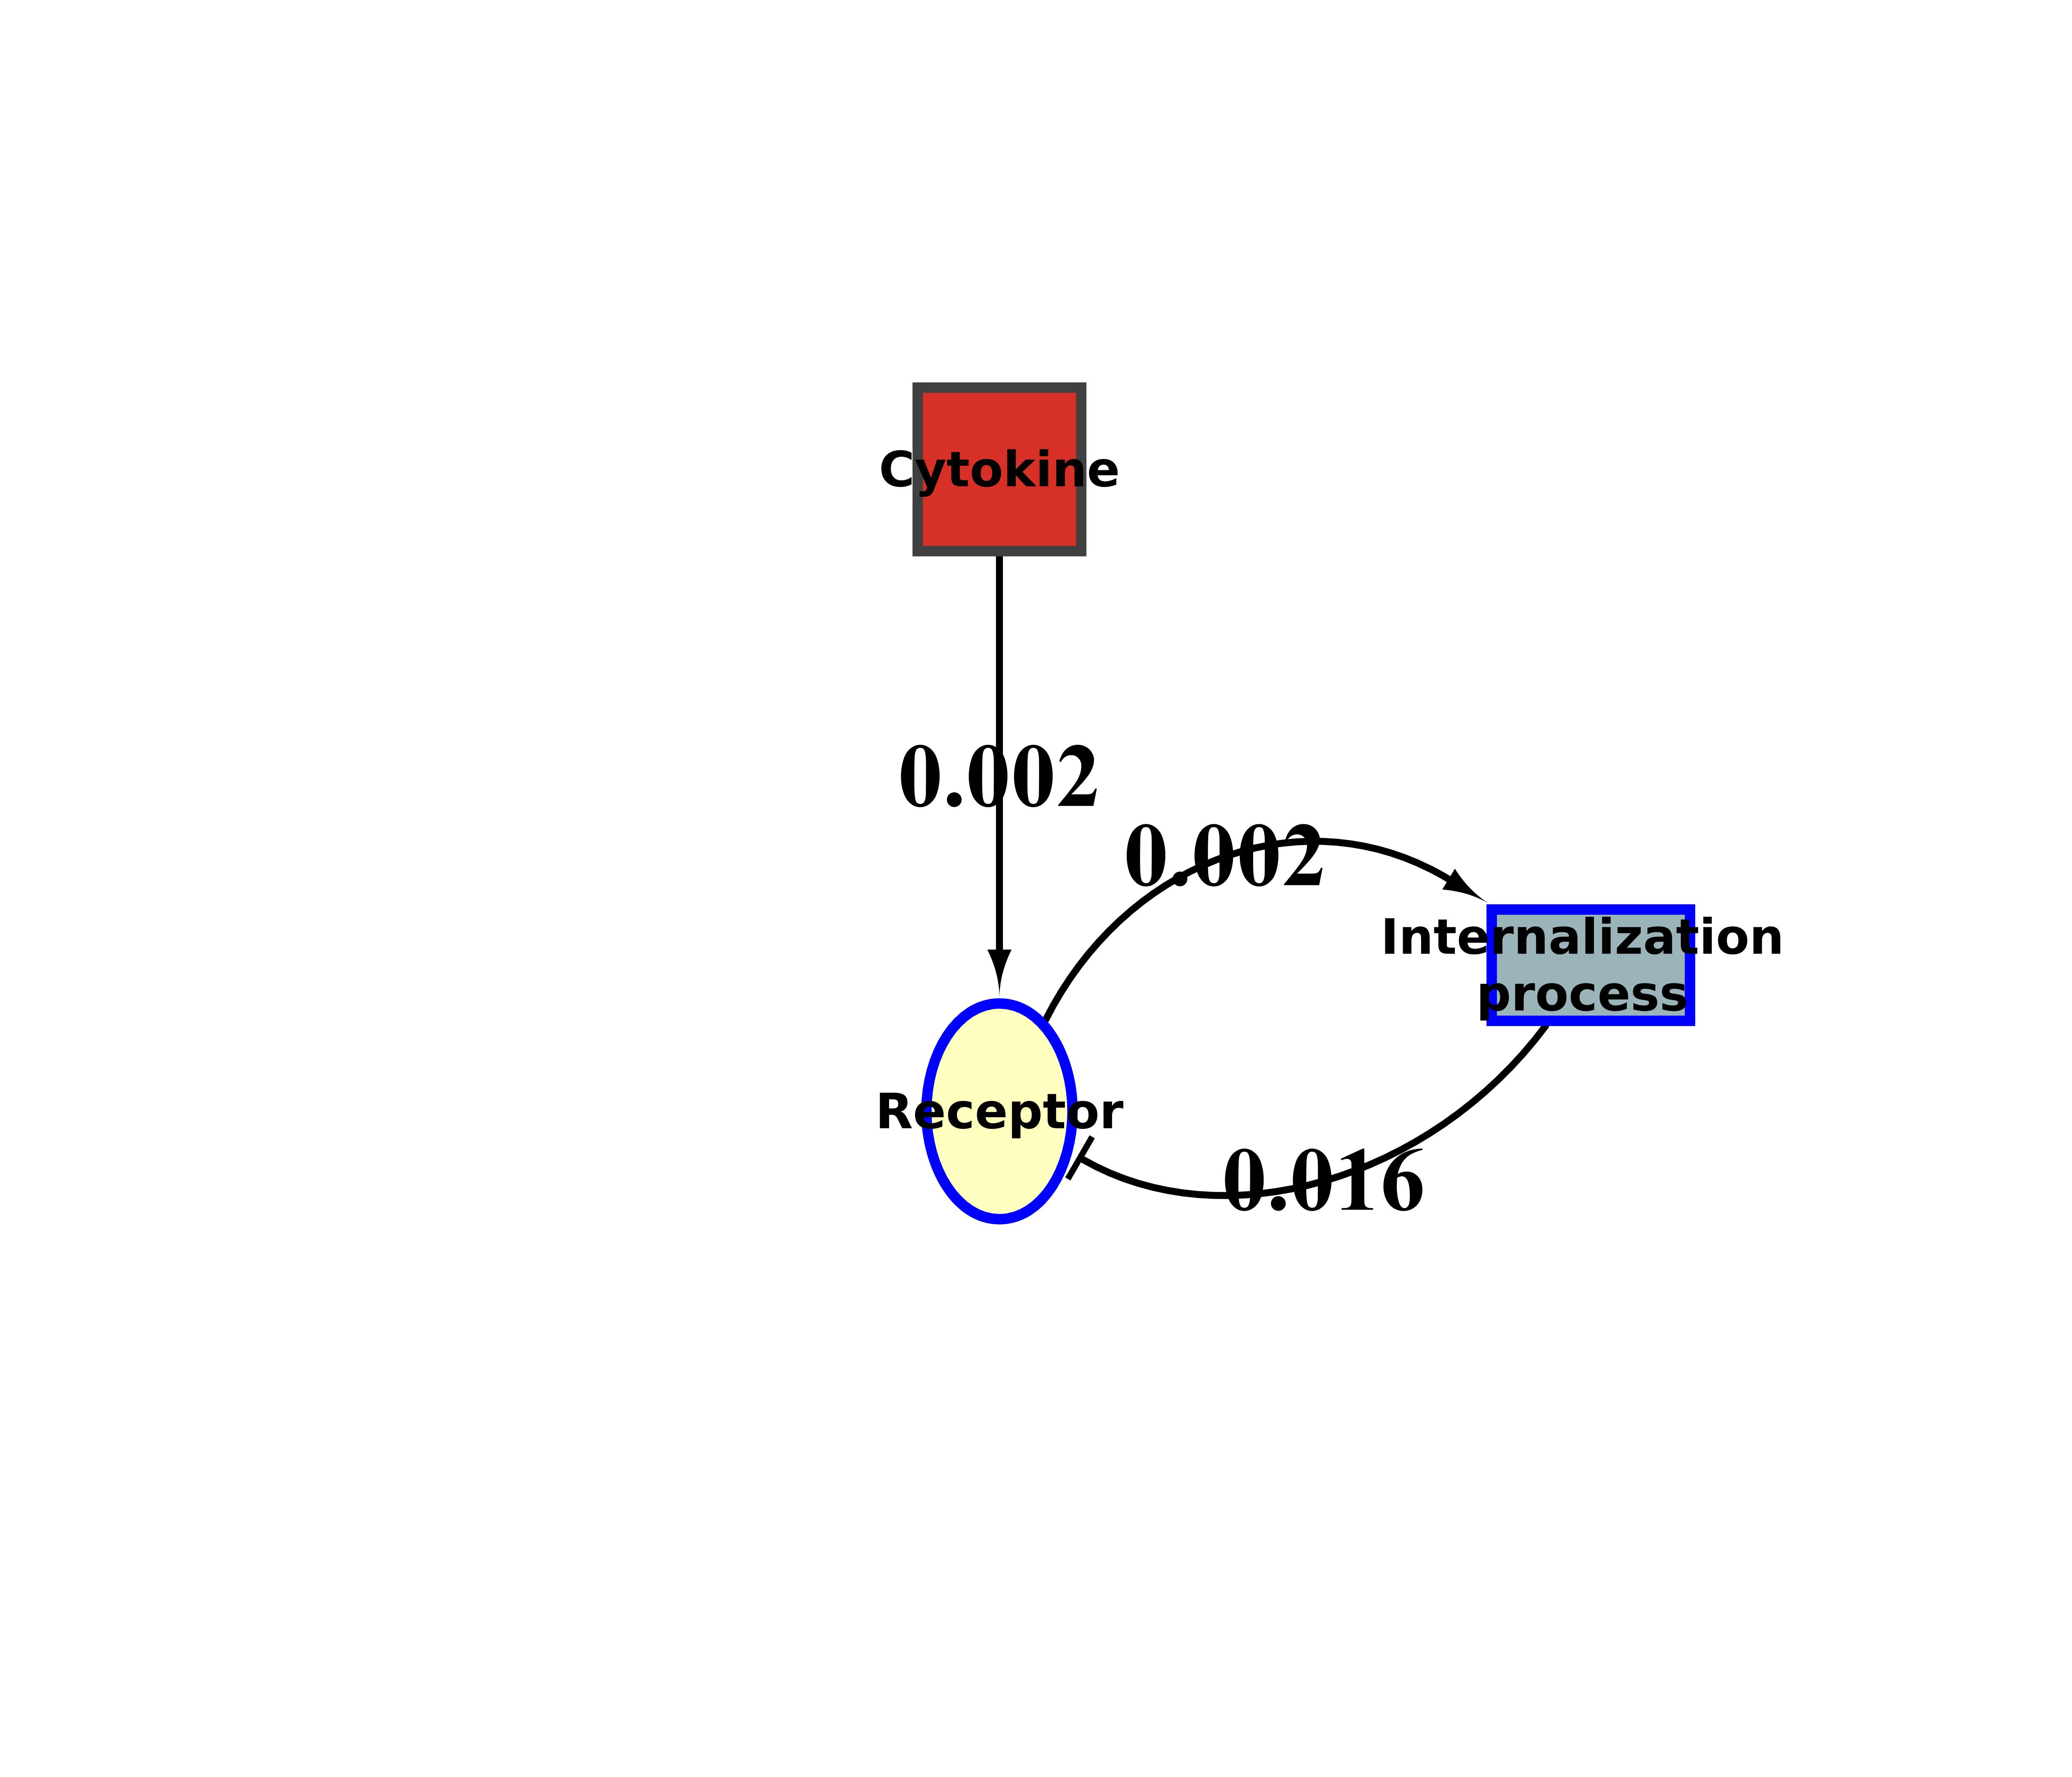
\includegraphics[scale=\graphScale]{feedback_network_CB}} & 
% \subfloat[\label{fig:animo-settings-feedback-graph}]{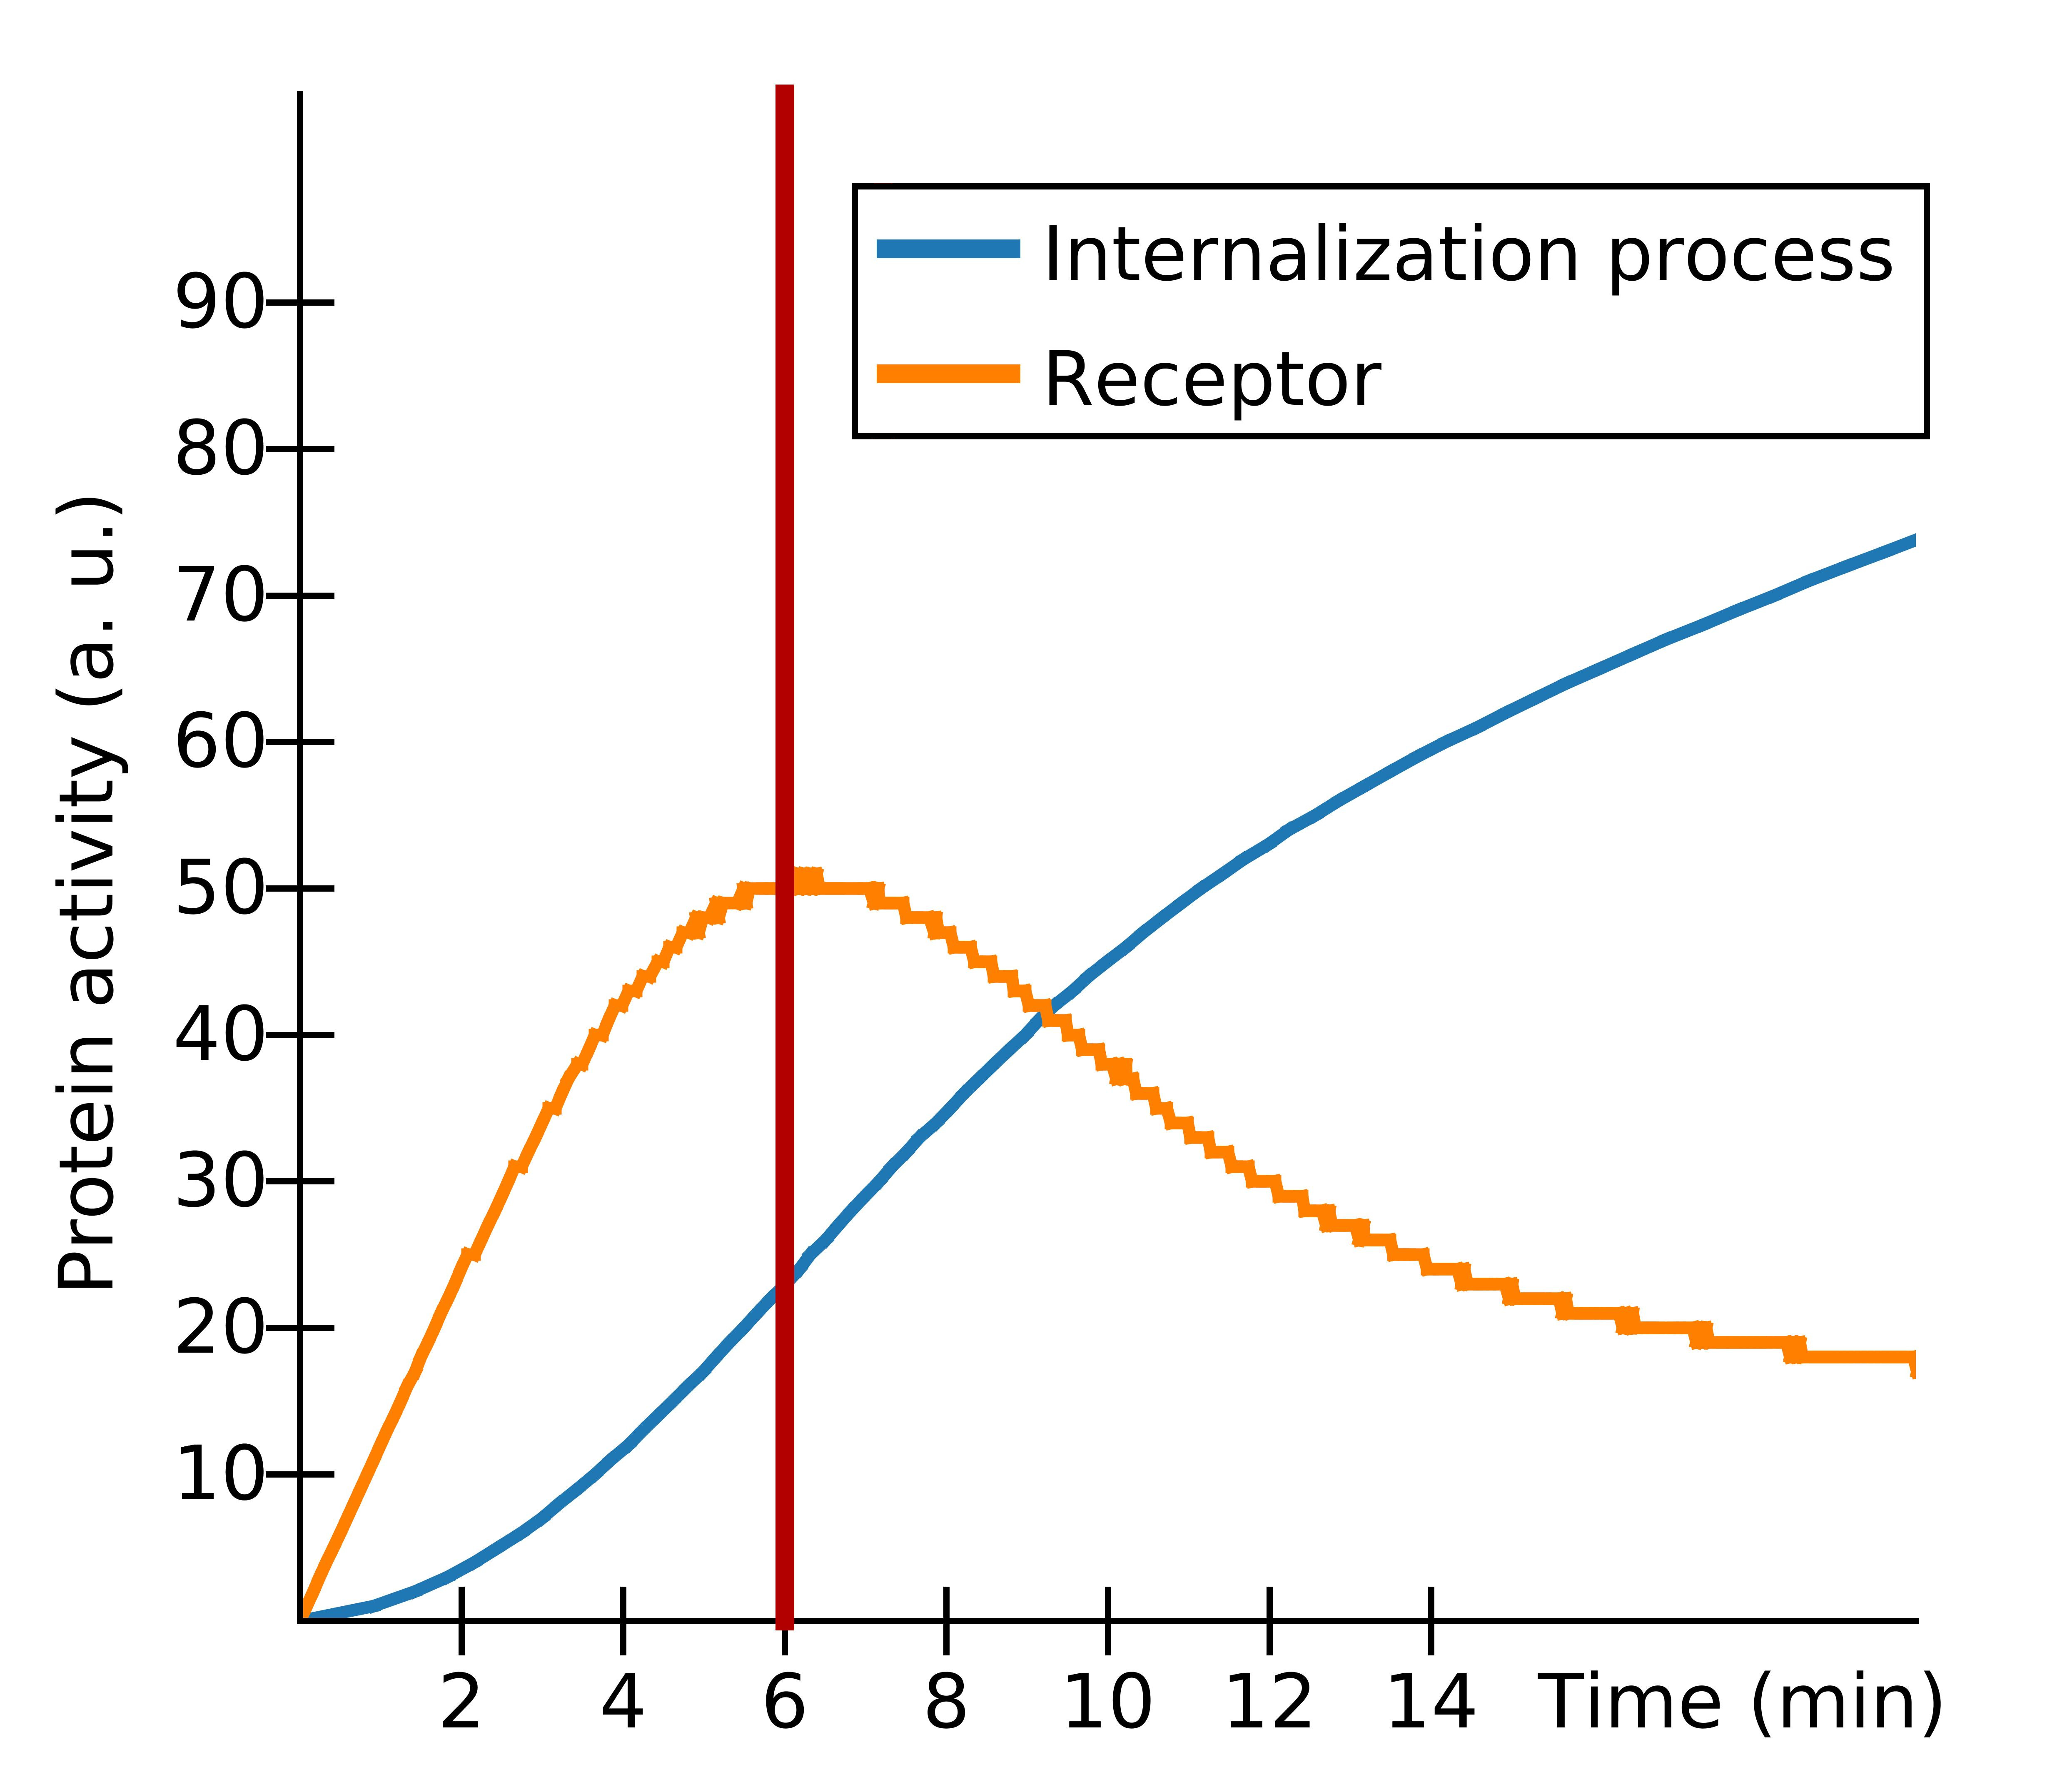
\includegraphics[scale=\graphScale]{feedback_graph}}
% \end{tabular}
% \caption{Example interaction settings for an ANIMO model. Each graph represents the time evolution
% of the network on its left. The vertical red lines in the graphs represent the point in time on which
% the coloration of the nodes in the corresponding network is based.\\
% {\bf ({\protect\subref*{fig:animo-settings-scenario-network}})} The two basic scenarios. Scenario 1
% makes the speed of the interaction depend only on the activity level of the upstream node {\sf Input}. In this case the
% upstream node is constantly active, so the activity of {\sf A} increases linearly with time. Scenario 2
% depends on the activity level of the {\sf Input} node, and on the \emph{inactivity} of {\sf B}. This
% makes the rate of activation of {\sf B} decrease proportionally to the current activity level of {\sf B}:
% the more {\sf B} is active, the slower the activation process will occur.\\
% {\bf ({\protect\subref*{fig:animo-settings-k-network}})} Choosing a value for the scaling factor $k$. While all interactions here
% are based on scenario 2, the value of their parameter $k$ (written on the edges) determines the speed at which the downstream node
% is activated: a larger value of $k$ means a faster reaction.\\
% {\bf ({\protect\subref*{fig:animo-settings-direct-network}})} Relation between network topology and delays. In order to delay the activation process
% ensuing an external signal (node {\sf Input}), we can reduce the reaction speed by changing $k$ or
% adding an intermediate node. Introducing a slowly activated ($k = 0.001$) node between {\sf Input} and {\sf B} is enough to
% activate {\sf B} at a much slower rate than {\sf A}, even if the value of $k$ for the last step is left unchanged at $k = 0.004$.
% Increasing the parameter of the newly introduced reaction lets us fine tune
% the speed of the response, making the activation of {\sf C} faster than {\sf B}, but still slower than {\sf A}. We repeat the process
% of introducing a delay with nodes {\sf D} and {\sf E}: an additional intermediate node further reduces the response time.\\
% {\bf ({\protect\subref*{fig:animo-settings-feedback-network}})} Peak dynamics are often observed in experimental data.
% In order to have the activity level of a node increase and successively decrease, the simplest way is to model it with a feed-back loop.
% In the example, we model the internalization of a receptor following its activation. Note that the interaction {\sf Internalization
% process} $\dashv$ {\sf Receptor} is an inhibition: being based on scenario 2, it will reduce the activity of the {\sf Receptor} node with a rate proportional
% to the current activity of both involved nodes. Scenario 1 dynamics are sufficient to model the two activating reactions {\sf Cytokine} $\rightarrow$ {\sf Receptor}
% and {\sf Receptor} $\rightarrow$ {\sf Internalization Process}. Key to the peak dynamics is the fact that the inactivation of the {\sf Receptor} node
% is much faster (higher $k$ value) than its activation.
% \label{fig:animo-networks}}
% \end{figure*}



\subsection{Preparing experimental data for use with ANIMO}
The measurements obtained from the digital imaging analysis of the PP96 plates were stored in a spreadsheet.
We will now illustrate the process through which this raw data was normalized and rescaled
to make it suitable for working with ANIMO.

A spreadsheet with all the data generated by applying the following steps is available in the Supplementary Materials.

\subsubsection{Background subtraction}
In order to estimate the background noise in the data, three wells in each plate
were kept empty (blank wells). 
A value of background noise was calculated for each spot as the average value of that spot in the blank wells.
The background noise values were then subtracted from the data of the corresponding spots in all the other wells.

\subsubsection{Normalization}
As both the reference and the normalization HSP60 spots yielded inconsistent results,
we decided to normalize the data grouping them by treatment condition and using one plate as reference.
Plate 3 (C20A4 cell line) was chosen as reference, as it shared conditions with both the other plates (donor cells).
Two normalization groups were then defined, separating the data for IL-1B treatment in plate 1 from
the data for treatments with Wnt-3a and Wnt-3a + IL-1B in plate 2.
The two groups were associated to the corresponding two groups in plate 3.

For each of the five considered spots (Akt, ERK, GSK-3B, JNK1, p38),
the average of the data was computed over all time points in each group. These values were then divided
by the average of the corresponding data in plate 3, obtaining the normalization factor.
In two cases (JNK1 and p38) the treatment with Wnt-3a was not considered 
for the computation of the normalization factor, as the response in that case was
considerably lower than with the other two treatments.

At the end of this process, each of the five spots in plate 1 and plate 2 had their own normalization factor, while
all factors for plate 3 were equal to 1. Each data point was then divided by the corresponding normalization factor.

\subsubsection{Data scaling}
As ANIMO models are semi-quantitative, it is not required to precisely estimate the molecular concentrations
in experimental data. For this reason, we rescaled all time series on a 0-100 interval,
dividing all the values by their maximum over a normalization group. For instance,
the scaled value for ERK in plate 2 is obtained dividing each normalized value by
the maximum normalized value of ERK over the two treatment conditions Wnt-3a and Wnt-3a + IL-1B in plate 2.

\subsubsection{Average series}
As the experiments were done in triplicate, three time series are available
for each treatment and spot. The time series we use as reference in our ANIMO models
contain average and standard deviation values over the triplicate values.

\section{Results}\label{sec:results}
\input{results.tex}

\section{Discussion}\label{sec:discussion}
\input{discussion.tex}

\section{Conclusions}\label{sec:conclusions}
\input{conclusions.tex}

%% The Appendices part is started with the command \appendix;
%% appendix sections are then done as normal sections
%% \appendix

%% \section{}
%% \label{}

%% References
%%
%% Following citation commands can be used in the body text:
%%
%%  \citet{key}  ==>>  Jones et al. (1990)
%%  \citep{key}  ==>>  (Jones et al., 1990)
%%
%% Multiple citations as normal:
%% \citep{key1,key2}         ==>> (Jones et al., 1990; Smith, 1989)
%%                            or  (Jones et al., 1990, 1991)
%%                            or  (Jones et al., 1990a,b)
%% \cite{key} is the equivalent of \citet{key} in author-year mode
%%
%% Full author lists may be forced with \citet* or \citep*, e.g.
%%   \citep*{key}            ==>> (Jones, Baker, and Williams, 1990)
%%
%% Optional notes as:
%%   \citep[chap. 2]{key}    ==>> (Jones et al., 1990, chap. 2)
%%   \citep[e.g.,][]{key}    ==>> (e.g., Jones et al., 1990)
%%   \citep[see][pg. 34]{key}==>> (see Jones et al., 1990, pg. 34)
%%  (Note: in standard LaTeX, only one note is allowed, after the ref.
%%   Here, one note is like the standard, two make pre- and post-notes.)
%%
%%   \citealt{key}          ==>> Jones et al. 1990
%%   \citealt*{key}         ==>> Jones, Baker, and Williams 1990
%%   \citealp{key}          ==>> Jones et al., 1990
%%   \citealp*{key}         ==>> Jones, Baker, and Williams, 1990
%%
%% Additional citation possibilities
%%   \citeauthor{key}       ==>> Jones et al.
%%   \citeauthor*{key}      ==>> Jones, Baker, and Williams
%%   \citeyear{key}         ==>> 1990
%%   \citeyearpar{key}      ==>> (1990)
%%   \citetext{priv. comm.} ==>> (priv. comm.)
%%   \citenum{key}          ==>> 11 [non-superscripted]
%% Note: full author lists depends on whether the bib style supports them;
%%       if not, the abbreviated list is printed even when full requested.
%%
%% For names like della Robbia at the start of a sentence, use
%%   \Citet{dRob98}         ==>> Della Robbia (1998)
%%   \Citep{dRob98}         ==>> (Della Robbia, 1998)
%%   \Citeauthor{dRob98}    ==>> Della Robbia


%% References with bibTeX database:

\bibliographystyle{model2-names}
\bibliography{Gene}

%% Authors are advised to submit their bibtex database files. They are
%% requested to list a bibtex style file in the manuscript if they do
%% not want to use elsarticle-harv.bst.

%% References without bibTeX database:

% \begin{thebibliography}{00}

%% \bibitem must have one of the following forms:
%%   \bibitem[Jones et al.(1990)]{key}...
%%   \bibitem[Jones et al.(1990)Jones, Baker, and Williams]{key}...
%%   \bibitem[Jones et al., 1990]{key}...
%%   \bibitem[\protect\citeauthoryear{Jones, Baker, and Williams}{Jones
%%       et al.}{1990}]{key}...
%%   \bibitem[\protect\citeauthoryear{Jones et al.}{1990}]{key}...
%%   \bibitem[\protect\astroncite{Jones et al.}{1990}]{key}...
%%   \bibitem[\protect\citename{Jones et al., }1990]{key}...
%%   \harvarditem[Jones et al.]{Jones, Baker, and Williams}{1990}{key}...
%%

% \bibitem[ ()]{}

% \end{thebibliography}

\end{document}

%%
%% End of file `elsarticle-template-harv.tex'.
